\documentclass{article}
\usepackage{float}
\usepackage{graphicx} 
\usepackage[
    backend=biber,
    style=alphabetic,
    sorting=ynt
]{biblatex}
\addbibresource{lib.bib}
\usepackage{subfig}
\usepackage[export]{adjustbox}
\usepackage{url}
\usepackage{pgfplots}
\usepackage{gensymb}
\usepackage{amssymb}
\usepackage{amsmath}
\usepackage{booktabs}
\usepackage{soul}
\usepackage[a4paper, total={6.5in, 9in}]{geometry}
\pgfplotsset{width=10cm,compat=1.9}

\title{A Computational Analysis of a Novel Chromatic k-Nearest Neighbours Algorithm}
\author{Thomas van der Plas, Frank Staals, Erwin Glazenburg}
\date{10 November 2024}

\newtheorem{theorem}{Theorem}
\newtheorem{lemma}[theorem]{Lemma}
\newtheorem{corollary}{Corollary}[theorem]
\newtheorem{observation}{Observation}[theorem]

% things that still are todo
\newcommand{\todo}[1]{{\color{red}[#1]}}
% things changes after first feedback round
\newcommand{\fb}[1]{{\color{blue}#1}}
\newcommand{\fbrm}[1]{{\color{blue}\st{#1}}}
\newcommand{\fbnote}[1]{{\color{blue}[FEEDBACK NOTE: #1]\\}}

\DeclareMathOperator{\polylog}{polylog}


\begin{document}

\maketitle

\begin{abstract}
    \fb{Classification algorithms are used in order to make predicitions based on historically available data. Chromatic $k$-Nearest Neighbour algorithms are an example of this, in which the} the color of a query point is determined by the mode color of its $k$ closest neighbours \fb{in historical data}. Classical approaches to solving this problem have a runtime which is dependent on $k$ or the amount of unique colors $c$. \fb{We investigate the computational performance of an alternative solution method proposed by van der Horst et al. in 2022 in which runtime is only dependent on the number of points in the historical dataset $n$. This should yield better performance when $k$ or $c$ are close to $n$.}\\
    We consider both range and mode finding in 1D and 2D contexts with a $L_\infty$ distance metric, comparing to a naive $k$ dependent implementation. We found that significant performance gains can be achieved from $k \gtrsim 300$ in 1D and $k \gtrsim 0.01n-0.1n$ in 2D, validated against both artificial and real life data points.
\end{abstract}

\section{Introduction}
\fb{
    Classification algorithms are widely used in order to make predictions about new data points based on historical data. In general, a query point $q$ is compared to a collection $P$ of $n$ existing data points with known classes. The class of $q$ is then determined by considering the classes of points in $P$ which are similar to $q$. Different algorithms apply different similarity metrics and techniques in order to determine what class is the most likely fit for our query. \\\\
    One widely used example of a classification algorithm is that of $k$-Nearest Neighbours ($k$-NN). In this, the $k$ points which are closest to $q$ are considered. From this set, the mode (or most frequently occuring) class is selected as a prediction for the class of $q$. When modeling this as a geometric problem, generic class labels are often replaced with colors. Additionally, data points are represented as points in $d$-dimensional space. This version is generally known as a Chromatic $k$-Nearest Neighbours algorithm. \\\\
    We are currently aware of only two results on the theory of chromatic $k$-NN algorithms. The first of these two is attributed to by Mount et al. \cite{MOUNT200097}. They introduced an approach using linear space datastructures that are able to answer theories efficiently if colors within $P$ are packed close together. For this, they devised a metric which they refer to as the chromatic density $\rho$ which allowed them to get a query time of $O(\log^2 n + (1/\rho)^d\log(1/\rho))$.\\
    The second result is attributed to van der Horst et al. \cite{vanderhorst_et_al:LIPIcs.ESA.2022.67}. Their goal was to introduce a set of algorithms that with near-linear space usage could answer queries with a running time only dependent on $n$. They note that this would be especially advantagous in the event that either $k$ or the amount of unique colors in $P$ are close to $n$. \\
    Our goal for this research is to get a better understanding of the advantages of having query times that are only dependent on $n$. We do this by implementing a selection of the algorithms presented in van der Horst et al. and comparing these with implementations of naive approaches. \\\\
    Van der Horst et al. proposed a selection of different algorithms. They provide exact approaches for solving in 1, 2, or $d$ dimensions with $L_2$, $L_\infty$ and $L_m$ distance metrics. They additionally provide approximation algorithms for $d=1$ and $d=2$ with a decreased runtime. In this research we will limit ourselves to implementing the exact $L_\infty$ approaches in both 1D and 2D. This selection was made as it provides a good base going forward. The 1D case provides us with the smallest possible instance of this problem, in which points are simply represented on a number line. The 2D case on the other hand forms the basis of the exact $d$-dimensional approach that was proposed, thereby allowing it to serve as a test of the real world applicability of the algorithm as a whole. \\\\
    Each of the algorithms proposed by van der Horst et al. is split into two major steps. The first of these is range finding, in which the $k$th closest point from $q$ is determined. This allows us to determine a radius from $q$ in which all points lie that need to be considered. After this we apply mode finding, in which given $q$ and our previously determined radius, we determine the mode color of the $k$ closest points to $q$. This second step allows us to answer our query. \\
    Following this two step split, we attempt to implement 4 seperate algorithms: 1D range finding, 1D mode finding, 2D range finding and 2D mode finding. Of these, we implement the first three as described by the original paper. 2D mode finding on the other hand could not directly be implemented as originally described; the preprocessing of this algorithm requires arrangements of planes to be built in 3D, however as far as we are aware major geometric computation libraries currently do not support this feature. As a result, we alter the original algorithm in order to only require arrangements in 2D. The underlying mechanisms of the algorithm are preserved, however due to this adjustment we can no longer answer mode queries for a certain radius. Instead, a halfplane mode query can be answered. We note that once 3D arrangements become available in geometric computation libraries, the groundwork that we laid down now should be easily adaptable allowing for radius based mode queries. We will therefore analyse the runtime of the implemented algorithm just as with the other 3 that were implemented without alteration. \\\\
    \fbnote{Based on Frank's feedback: I wanted to still fully split 2D range finding and 2D mode finding, however I didn't have the time to fully seperate the two as that would require major rewrites of certain parts. Current setup isn't ideal, however I hope it is clear enough to a reader that the mode is a halfplane query.}
    The structure of this paper will be as follows. For all sections except the conclusion, we will seperate the 1D and 2D implementations. In this, we will split further by discussing range and mode finding operations seperately.\\
     In Section 2, we will provide a summary of all the algorithms that were implemented. This also includes the naive approaches that were included as benchmarks for our results. In Section 3, we will discuss implementation details for each of the algorithms derived from van der Horst et al. Here we also discuss any possible modifications that were made in order to make algorithms computationally feasible. In Section 4, we discuss the test instances that we used and the results that our implementation produced. Then finally in Section 5, we will conclude, reflect and provide an overview of possible future work. 
}
\section{Methods}
Here, we provide an overview of the computational complexities and outlines of
the algorithms implemented in this paper. Only brief summaries of the vital
parts of algorithms are provided; for more details, we refer the reader to the
original work or to the source code in which the algorithms are implemented. An
overview of all runtimes and space usage of the algorithms can be found in
Table \ref{tab:runtimes}.
\begin{table}[h]
    \centering
    \begin{tabular}{llll}
        \toprule
        Algorithm   & Preprocessing time & Space         & Query time                 \\
        \cmidrule(lr){1-1}\cmidrule(lr){2-4}
        1D $L_{m}$ Naive range & $O(n \log n)$      & $O(n)$        & $O(\log n + k)$            \\
        1D $L_{m}$ Fast range  & $O(n \log n)$      & $O(n)$        & $O(\log n)$                \\
        1D $L_{m}$ Naive mode  & \fb{$O(n \log n)$} & \fb{$O(n)$}   & \fb{$O(\log n + k)$}       \\
        1D $L_{m}$ Fast mode   & $O(n^{3/2})$       & $O(n)$        & $O(\sqrt{n})$              \\
        \addlinespace[0.6em]
        2D $L_{\infty}$ Naive range & \fb{-}      & \fb{$O(n)$}       & \fb{$O(n \log n )$}           \\
        2D $L_{\infty}$ Fast range  & $O(n \log n)$      & $O(n \log n)$ & $O(\log^2 n)$              \\
        2D $L_{\infty}$ Naive mode  & $\fb{O(n \log n)}$ & $O(n)$        & \fb{$O(\log n + k)$}       \\
        2D $L_{\infty}$ Fast halfplane mode   & $\fb{O(nr^2)^*}$   & $O(nr)^*$     & $\fb{O((n/r) \polylog n)}$ \\
        \bottomrule
    \end{tabular}
    \caption{Computational complexities of the implemented algorithms. * indicates a deviation from the reference material.}
    \label{tab:runtimes}
\end{table}
\subsection{1D}
\subsubsection{Naive range finding}
\textit{Preprocessing} ($O(n \log n)$ time, $O(n)$ space): Sort the pointset $P$, save this sorted list. \\\\
\textit{Query} ($O(\log n + k)$ time): Binary search to find the index of the point closest to the query point $q$ within the pointset $P$. Using this index $q_i$, then find the $k$th nearest point by stepping either left or right from $q_i$ in the index range $[q_i-k, q_i+k]$. \fb{Return the distance between $q$ and the $k$th nearest point.}
\subsubsection{Fast range finding}
Based on the algorithm described in section 2.1 of the paper by Van der Horst
et al. \cite{vanderhorst_et_al:LIPIcs.ESA.2022.67}. \\\\ 
\textit{Preprocessing} ($O(n \log n)$ time, $O(n)$ space): Sort the points, then save
points in a node-valued binary search tree $T$ that contains size annotations.
\\\\ \textit{Query} ($O(\log n)$ time): Based on the query point $q$, split $T$ into two trees
$T_{P^<}$ and $T_{P^{\geq}}$ that contain the points $< q$ and $\geq q$
respectively. Note that both these trees have their points ordered on distance
from $q$, however orderings are flipped between the two trees. \\ Now, let $R$
be the tree whose root is farther from $q$, and let $B$ be the other tree. For
$R$, let $r$ be its root, $R^<$ be the subtree containing elements closer to
$q$ and $R^>$ be the other tree. Let $B$ have identical definitions for $b$,
$B^<$ and $B^>$. Lastly, let $\ell = |B^<| + |R^<| + 1$. \\ Based on this
$\ell$, we now have two distinct cases. \fb{These are visualised in Figure \ref{fig:vanderHorst_treesplit}, which appeared as Figure 3 of van der Horst et al.} \\ 
$\ell \geq k$: target element is
not $r$ or in $R^>$; let $R \leftarrow R^<$\\ $\ell < k$: target element is not
$b$ or in $B^<$; let $B \leftarrow B^>$, and let $k \leftarrow k - (|B^<| +
    1)$. \\ After the modification of the trees has taken place, ensure that $r$ is
still farther from $q$ than $b$; if not, flip the assignments of $R$ and $B$ to
ensure this holds. Continue the process until one of the trees is a leaf, after
which the $k$th element can be found trivially using the size annotations.
\begin{figure}%
    \centering
    \includegraphics[width=12cm]{figs/opt_rank.pdf}
    \caption{\fb{(Sub)Trees that may contain the $k$th furthest point from $q$ during fast 1D range finding based on $\ell = |B^<| + |R^<| + 1$}}%
    \label{fig:vanderHorst_treesplit}%
\end{figure}
\subsubsection{Naive mode finding}
\textit{Preprocessing} ($O(n \log n)$ time, $O(n)$ space): \fb{Sort the pointset $P$, save this sorted list.} \\\\
\textit{Query} ($O(\log n + k)$ time): \fb{Based on $q$ and the provided radius, determine the indices into $P$ that fall within the radius around $q$ using a binary search for the lower and upper bound. Afterwards, count the frequency of each color within our index range using a dictionary. Return the color with the highest counted frequency.}
\subsubsection{Fast mode finding}
Based on the algorithm described in section 3 of the paper by Chan et al.
\cite{Chan2014}. \\\\ 
\textit{Preprocessing} ($O(n^{3/2})$ time, $O(n)$ space): Transform an array $\bar{A}$ in
which each entry contains a color in the range $[0, \Delta)$ into a set of
arrays $Q_a$ for $a \in [0, \Delta)$ such that $Q_a$ contains an ordered list
of indexes into $\bar{A}$ where $\bar{A}[i] = a$. Additionally, create an array
$\bar{A}'$ such that $\bar{A}'[i]$ is equal to the rank or index of $i$ in
$Q_{\bar{A}[i]}$. \\ Lastly, precompute the modes of spans of elements with
length $t = \sqrt{n}$. Do this by storing two tables $S$ and $S'$ each of size
$t \times t$ such that for any $0\leq b_i \leq b_j < t$, $S[b_i, b_j]$ contains
the mode color of $\bar{A}[b_it : (b_j + 1)t)$, and $S'[b_i, b_j]$ contains the
corresponding frequency. These precomputed spans can be determined using a
naive counting implementation. \\\\ 
\textit{Query} ($O(\sqrt{n})$ time): Given a query range $[i, j)$, calculate $b_i=\lceil i/t \rceil$ and $b_j=\lfloor j/t \rfloor - 1$,
representing the indices of the first and last precomputed spans fully within
the query range. Let the range $[i : \min{b_it, j})$ (in range elements before
the first precomputed span) be known as the prefix, and let the suffix be
defined similarly as $[\max{(b_j + 1)t, i} : j)$. \\ \fb{By Lemma 2 of the paper by Chan et al.} the mode of $\bar{A}[i,
    j)$ must either be an element in the precomputed range defined by $b_i$ and
$b_j$, or an element in the prefix or suffix. Let $c$ be the mode and $f_c$ the
corresponding frequency of the precomputed range. Now sequentially scan the
elements \fb{in} the prefix and suffix to see whether these candidates $c$ and $f_c$
need to be updated in order to represent the mode of the whole range $[i, j)$.
\\ Starting from the first element in the prefix, if the color has not yet been
considered, determine whether its frequency is at least $f_c$ by testing if
$Q_{\bar{A}[x]}[\bar{A}'[x] + f_c - 1] < j$, where $x$ represents the index of
the current element. If this is the case, determine the frequency $f_x$ of
$\bar{A}[x]$ in $[i, j)$ by doing a linear scan of $Q_{\bar{A}[x]}$ \fb{starting from $\bar{A'[x] + f_c - 1}$. Section 3.3 of their paper shows that this scan is performed in $O(t)$ time}. Our
candidate $c$ and $f_c$ can then be updated to be $c \leftarrow \bar{A}[x]$ and
$f_c \leftarrow f_x$.
\subsection{2D - $L_\infty$}
\subsubsection{Naive range finding}
\fbnote{I made a mistake here (as well as in the naive mode) by using a definition of $L_{\infty}$ that uses a \textit{minimum} instead of a \textit{maximum}. I don't really know how this happened. For the mode, I now made the naive case simply do a range tree query + color counting. For range finding on the other hand, I couldn't figure something out in time that was simpler than the algorithm already proposed while still having a decent (and ideally $k$ dependent) runtime. I therefore opted to use the most naive of all approaches by simply sorting all distances. I am aware that this is not an ideal baseline, however given the time this is the best I could still do. }
\fb{
\textit{Preprocessing} ($O(n)$ space): None, only saving the pointset $P$. \\\\
\textit{Query} ($O(n \log n)$ time): Determine the distance between all points in $P$ and $q$. Sort the list, and return the $k$th entry.
}
\subsubsection{Fast range finding}
Based on the algorithm provided in Section 3.1 of the paper by Van der Horst et
al. \cite{vanderhorst_et_al:LIPIcs.ESA.2022.67}.\\\\ 
\textit{Preprocessing} ($O(n \log n)$ time, $O(n \log n)$ space): Create a rangetree $R$ \fb{with size annotations} on our pointset $P$. Additionally, sort $P$ into two
arrays $A_x$ and $A_y$, where $A_x$ contains all points sorted on $x$
coordinates and $A_y$ contains all points sorted on $y$. \\\\ 
\textit{Query} ($O(\log^2 n)$ time):
Let $x_0, ..., x_\ell$ be the x-coordinates that are at most $q_x$. Let $x_i$
be one of these coordinates; let $r = q_x - x_i$. We can now find the amount of
points in the bounding square around $q$ defined by $x_i$ by doing a counting
query using $R$ with the range $[q_x - r, q_x + r] \times [q_y - r, q_y + r]$.
Using this count, binary search over $x_0, ..., x_\ell$ in order to find the
bounding box with smallest $r$ that contains at least $k$ points. Repeat for
the $x$ coordinates greater than $q_x$ as well as the smaller and larger $y$
coordinates, then return the smallest $r$.
\subsubsection{Naive mode finding}
\fb{
\textit{Preprocessing} ($O(n \log n)$ time, $O(n \log n)$ space): Create a rangetree $R$ on our pointset $P$. \\\\
\textit{Query} ($O(\log n + k)$ time): Given a radius $r$, query $R$ for the points in $[q_x - r, q_x + r] \times [q_y - r, q_y + r]$. Determine the mode color of these points by counting using a dictionary and returning the color with highest frequency. 
}
\subsubsection{Fast halfplane mode finding}
\textbf{Note: } the algorithm provided here does \textit{not} find the mode of a k-nearest neighbour query; it instead returns the mode color of a halfplane query. More details on the algorithm and the reason for this choice are provided in Section 3.2. \\
Adapted from the algorithm provided in Section 4.2 of the paper by Van der Horst et al. \cite{vanderhorst_et_al:LIPIcs.ESA.2022.67}. \\\\
\fbnote{For this section, all mention of face $f$ has been replaced with face $a$ in order to reduce confusion with frequencies $f_x$.}
\textit{Preprocessing} ($O(nr^2)$ time, $O(nr)$ space): Let $L$ be the set of dual lines corresponding to our initial pointset $P$. \fb{Using a random subset $L_{\mathcal{A}}$ of $r \log r$ lines in $L$, create an arrangement $\mathcal{A}$ and triangulate it. By Theorem 14 of Chazelle and Friedman \cite{21970}, $\mathcal{A}$ has a constant probability of being a $1/r$ cutting of $L$. If it is not, retry with different sets $L_{\mathcal{A}}$ until a $1/r$ cutting $\mathcal{A}$ is found.}\\ A conflict list $C$ can then be constructed, in which for each face $a$ in $\mathcal{A}$, $C_a$ stores references to all lines in $L$ that intersect that face. If the maximum amount of lines intersecting a faces is more than $n/r$, the cutting is rejected and we start over, otherwise we accept the cutting. \\
\fb{Precompute a trapezoidal decomposition $\mathcal{T}$ of $\mathcal{A}$ in order to answer point queries efficiently. Annotate each face $a$ in $\mathcal{A}$ in order to store the mode color $m$ and corresponding frequency $f_m$ of the colors of $C_a$. Additionally, let $L_a$ be the set of lines that lie fully below a face $a$. Add the frequency $f_c$ in $L_a$ of any color $c$ that occurs both in $L_a$ as well as $C_a$ to our annotation of $a$ as well.}\\\\
\textit{Query} ($O((n/r) \polylog n)$ time): Given a halfspace $h$ in our primal space, transform it to its point dual $q_h$. Find the face $a$ that contains $q_h$ by performing a point location query on $\mathcal{T}$. Using the annotations on the face $a$ and the conflict list $C_a$, count the colors of the lines in $C_a$ that are below $q_h$. Combine these with the precomputed frequencies $f_c$, and return the mode.
\section{Implementation details}
In this section, we discuss implementation details for the selected algorithms
along with modifications made to the reference material used in order to make
implementation easier. All algorithms were implemented in C++11 due to low
computational overhead and support for existing libraries containing base
geometric algorithms. The implementation itself is freely available on GitHub,
along with tools for generating test instances \cite{vanderPlasImplementation}.
\subsection{1D}
Large parts of the work of Van der Horst et al.
\cite{vanderhorst_et_al:LIPIcs.ESA.2022.67} were directly implemented, however
two elements of note were adapted from the original source material in order to
make computation easier and feasible. These were 1) the tree splitting that is
required for the range finding operation, and 2) certain details of the fast
mode finding algorithm described by Chan et al. \cite{Chan2014}.
\begin{figure}%
    \centering
    \subfloat[\centering Initial tree with search path and split highlighted]{{\includegraphics[width=4cm]{figs/fig1.eps} }}%
    \qquad
    \subfloat[\centering Trees after split]{{
\includegraphics[width=6cm]{figs/fig2.eps} }}%
    \caption{Splitting process on part of balanced binary search tree for $q=68$. Subtrees unaffected by the split are represented as triangles.}%
    \label{fig:example}%
\end{figure}
\subsubsection{Tree splitting}
Van der Horst et al. requires that the initial ordered tree of points is split
into two halves \cite{vanderhorst_et_al:LIPIcs.ESA.2022.67}: one containing all
points $\geq q$, and one containing all points $< q$. This operation must be
performed in $O(\log n)$ in order to maintain the given time complexity of the
algorithm. A red-black tree is offered as one possible solution to do this in
$O(\log n)$ time, however in practice this is complicated to implement and a
computationally heavy operation.\\\\ As a sidenote in the original paper, it is
mentioned that with some care the same operation could also be performed using
a balanced binary search tree. Implementation details for this split operation
are however not described. As this still seemed like the better of the two
options, we decided to go with this route, and have provided both a methodology
for this split as well as a proof of its functionality and time complexity. An
illustration of this splitting operation has been provided in Figure
\ref{fig:example}. \\\\ Let $T$ be a node-valued balanced binary search tree
containing the points $P$ (where $n = |P|$), and let $q$ be the query point.
Additionally, let $S = [(t_1, d_1), ..., (t_s, d_s)]$ be the search path that
is traversed when searching for $q$ in $T$, where $t$ represents a node that is
visited, and $d$ represents the direction in which the search is continued from
$t$ (either left or right). As the search stops at $t_s$, let $d_s$ be the
direction in which the search would have continued if $t_s$ had child nodes.
Our goal is to create two binary search trees $L$ and $R$ such that $L$
contains all points $<q$, and $R$ contains all points $\geq q$. Furthermore,
the height of both $L$ and $R$ must be at most $O(\log n)$. \\\\ Using our
search path $S$, we can split T. Let $l$ and $r$ be references to the largest
node in $L$ and smallest node in $R$ respectively, and let them both be
initialized as a leaf. Furthermore, during \fb{our} process if $l$ or $r$ are not
\fb{themselves} leaves, let \fb{us require that} $l.right$ and $r.left$ respectively be a leaf. Now, starting from
$(t_1, d_1)$, first determine on which side of the tree the node $t_1$ will be
appended. In general, if a $d_i$ is right, its corresponding $t_i$ must be part
of the $L$ and vice versa. Without loss of generality, we will assume that
$d_i$ is right in our discussion of how to append $t_i$ to its split tree. \\\\
In order to add $t_i$ to $L$ whilst constructing a tree that is still valid
binary search tree, we wish to maintain that \\ 1) $L$ only contains points $<
    q$ \\ 2) $L$ is sorted \\ 3) $l$ is the largest node currently present in $L$
\\ 4) $l.right$ is a leaf if $l$ is not a leaf \\ In order achieve this, we
consider two distinct cases: \\\\ \textit{If $l$ is still a leaf}, we can
maintain the desired properties by setting $t_i.right \leftarrow leaf$, $l
    \leftarrow t_i$; all four properties follow trivially from our operation, as
$t_i.left$ by definition of a binary search tree could only contain values
smaller than $t_i$ and no further reordering is done. \\ \textit{Otherwise},
$l$ must by our previous definition already be a node with $l.right = leaf$,
and by definition of $L$ we must have gone right in our search path after
visiting $l$. We therefore know that $t_i$ must be larger than $l$.
Additionally, as $t_i$ is part of the same search path as $l$, all elements in
$t_i.left$ must be larger than $l$ while being smaller than $t_i$. If we
therefore set $t_{\fb{i}}.right \leftarrow leaf$, $l.right \leftarrow t_{\fb{i}}$, followed by
updating our reference to $l$ by setting $l \leftarrow t_{\fb{i}}$ we know that once
again all properties hold. This same process can be applied when $d$ is left by
flipping all directions and references to $l$ and $L$ with $r$ and $R$
respectively. \\\\ By doing this, we create two trees $L$ and $R$ which
maintain their sorted property. We also know that no nodes are lost in this
process, as the child that is set to be a leaf during our iterations also is
the next node considered for appending to either tree, thereby including it.
Furthermore, by definition of a balanced binary search tree, we know that the
$i$th node in the search path in $T$ can have a height of at least $\log n - i$
and at most $\log n - i + 1$. Any additions of nodes are always done on an
empty side of a node which came previously in the search path; the height of
the non-empty side was therefore at least $\log n - i$. Using this we can
conclude that over a maximum of $\log n$ additions, the overall height of the
tree remains $O(\log n)$.\\ Lastly, in this process only the children of the
nodes in the search path are modified. Saving the original nodes in a seperate
datastructure such as an array thus allows us to revert the process in $O(\log
    n)$ time by replacing the nodes in the search path. With this, the following
lemma follows: \\
\begin{lemma}
    In $O(\log n)$ time, we can split a balanced binary search tree $T$ with $n$ nodes along a query point $q$ into two binary search trees $L$ and $R$, where $L$ contains all points $<q$ and $R$ contains the points $\geq$ q. Furthermore, both $L$ and $R$ have a height at most $O(\log n)$, and the splitting operation can be reverted in $O(\log n)$ time.
\end{lemma}
The implementation of the algorithm described by Van der Horst et al. also requires size annotations in each of the tree nodes. In this, we note the following observation:
\begin{observation}
    When splitting $T$ into $L$ and $R$, the size of a node only changes if that node is part of a search path.
\end{observation}
This follows from the fact that only nodes in the search path have their children modified during the splitting process; As the size of one child does not influence the size of its sibling, we can also conclude that this effect remains limited to the nodes among the search path. \\\\
It is therefore possible to both set and revert the new sizes of the nodes in the split trees $L$ and $R$ in $O(\log n)$ time, allowing us to extend our previous Lemma:
\begin{lemma}
    In $O(\log n)$ time, we can split a balanced binary search tree $T$ with $n$ nodes and size annotations along a query point $q$ into two binary search trees $L$ and $R$, where $L$ contains all points $<q$ and $R$ contains the points $\geq$ q. Furthermore, both $L$ and $R$ have a height at most $O(\log n)$, and the splitting operation can be reverted in $O(\log n)$ time.
\end{lemma}
Using this Lemma, we can conclude that it is indeed possible to replace the recommended red-black tree with an in place modified balanced binary search tree.

\subsubsection{Fast mode finding}
The algorithm described by Chan et al. \cite{Chan2014} was used by Van der
Horst et al. in order to achieve a $O(\sqrt{n})$ mode query time with $O(n)$
storage. For this, the first algorithm described in section 3 of Chan et al.
\fbrm{their publication} suffices. During implementation of this, a few things of note
were changed.\\\\ Firstly, the array $A$ (and its derivatives) containing all
colors were changed from being 1-indexed to being 0-indexed. While this does
not have any effect on the functionality or runtime of the algorithm itself, it
is noted that some details might differ between the reference description and
the eventual implementation as a result. The summary of the algorithm that was
provided in Section 2 has already been updated to reflect this change in
indexing.\\\\ Secondly, in section 3.2 of Chan et al.\fbrm{'s publication,} two
indices are calculated: these indices, called $b_i$ and $b_j$, represent the
index of the first and last precomputed mode span respectively in the
datastructure $S$. These are subsequently used in order to determine the mode
color of the precomputed part of the query span. We note however that if a
query is fully contained within a single precomputed span, these indexes either
represent an empty range, or are invalid. \\ In these cases, a fallback to the
naive counting implementation was added instead. We note that this does not
change the time complexity of the overall algorithm, as the size of a
precomputed span is at most $\sqrt{n}$, therefore any fallback will still run
in $O(\sqrt{n})$ time. We additionally note that this implementation also
prevents $b_j$ from becoming a negative index in the event that the end of the
query span is in the first precomputed span.
\subsection{2D}
The 2D algorithms described in van der Horst et al. required the use
of several well known geometric datastructures and algorithms. As implementing
these is prone to subtle issues, requires a significant level of expertise and
is generally a lot of work, the decision was made to use an existing library to
act as a supporting framework. CGAL 6.0 \cite{cgal:foundations} was selected
for this, as it provides most of the datastructures and querying algorithms
that we will need to proceed. This allowed us to focus on the novel ideas
proposed in the paper. \\\\ For range finding, Van der Horst et al. their
description for the algorithm could once again be followed. Mode finding on the
other hand could not directly be implemented. The reason for this was a
limitation in CGAL itself. The original intent was to
use the library in order to generate 3D arrangements from planes, as this forms
the basis of the precomputed datastructure used for answering queries in the
original work. When initially selecting this library however, we failed to
notice that only 2D arrangements were supported. The decision was therefore
made to implement a alternate version of the mode query which works on query
halfplanes instead. \fbnote{As a response to Erwin's feedback: Emphasis on this was added in the introduction as this was recommended by Frank.}
\\\\ The alternate version uses much of the same machinary
seen in the original, however it has been adjusted to work with 2D arrangements
instead. By providing this alternate version, we hope to both get a general
idea of the performance of mode queries using this basis, as well as providing
a framework which can be expanded upon when 3D arrangements can be easily made. \\\\
\fb{
    A last thing of note is that the introduction of a second dimension can lead to degeneracies such as duplicate x or y coordinates. Due to time constraints, no expansive validation was performed to ensure that our implementation could handle all edge cases caused by this. As a workaround, datapoints are slightly offset in order to discourage degeneracies from forming.
}
\subsubsection{Fast range finding}
As noted before, the range finding algorithm was directly implemented as
described by Van der Horst et al. The method requires the use of a range tree
for counting queries. Range tree implementations are widely available,
therefore one was selected that matches our algorithmic requirements. As we aim
to fully remove dependency on $k$ and aim to match the runtime described in the
original paper, a range tree that supports fractional cascading and native
counting queries was required. CGAL, the library used for most of the base
geometric algorithms in 2D mode finding, has a $d$-dimensional range tree with
fractional cascading \cite{cgal:rangetree}. It however sadly does not support
native counting queries, therefore the use of this would introduce dependency
on $k$ as iterating over output points is required. \\\\ An alternative was
found in an open source project by Weihs, which implemented $d$-dimensional
range trees based on doubles \cite{Lucaweihs}. As we wanted to integrate these
results with the CGAL implementation used in mode finding, the range tree
implemented by Weihs was modified in order to support native CGAL points
\cite{cgal:numbertypes} \cite{cgal:foundations} \cite{cgal:dDkernel}.

\subsubsection{Fast mode finding}
A 2D arrangement version of the algorithm described by Van der Horst et al. was
created. In the original work, points are passed through a lifting operation in
order to create planes. A 3D arrangement using $r \log r$ of these planes can
then be created and triangulated, thereby creating a $1/r$ cutting of the dual
space with constant probability. They then show that a query point $q$ and
radius $r$ can be transformed into a point $q^*$ in the dual space, where the
mode of points within $r$ distance from $q$ can be found as the mode of the
planes below $q^*$ in the dual space. \\\\ In order to achieve a similar result
using only 2D arrangements, the lifting operation was replaced with a simple
point/line dual. This once again allows us to create a $1/r$ cutting in dual
space, where the lines below a point $q^*$ can be found using the same
mechanisms as in 3D. The query point $q^*$ now maps to a halfspace in the
primal space, therefore making this alternate algorithm a halfspace mode query.
\\\\ In order to generate face conflict lists and color frequencies per face as
mentioned in Section 2.2.4, a naive method was used which directly compares all
faces with all lines. The resulting preprocessing time is therefore $O(nr^2)$ as can be seen in Table \ref{tab:runtimes}, which is
greater than the theoretical runtime of \fb{$O(n^{1+\delta}+nr^3)$ described by van der Horst et al.} Due to storing
the entire conflict list and color frequencies instead of computing them at
runtime, our space requirement is also $O(nr)$ instead of the theoretical $O(n
    + r^3)$. Both of these could still be improved with a better implementation.
\\\\ CGAL was used for line and segment intersections, point representation, 2D
arrangement creation and annotation and trapezoidal decompositions of the
arrangement for point location queries \cite{cgal:foundations}
\cite{cgal:numbertypes} \cite{cgal:arrangement}. The rest of the required
datastructures and operations were implemented using features natively
available to C++11.
\section{Computational results}
In this section, we aim to provide an overview of the test instances used to
validate performance of the implemented algorithms. Additionally, performance
graphs are shown for artificial as well as real life based instances. For a
full overview of unformatted results, we refer the reader to the Appendices.
\\\\ All results were measured using C++11 in Visual Studio on Windows in
release mode using default compiler settings, and run on a Intel i7-10750H CPU
using 40GB of RAM.
\subsection{1D}
For 1D, both artificial and real life data \fb{are} used in order to perform
computational experiments. The use of artificial data for this section \fb{is} largely due to the fact that real life data often has more than a single
dimension, making the acquisition of a comprehensive dataset difficult.
Some real life data \fb{is} included in order to validate the results that were
achieved in the artificial counterpart, however this \fb{is} based on an originally
2D dataset which \fb{is} projected in order to match our requirements.
\subsubsection*{Artificial data} Both the naive and tree-based range finding
approaches are not dependent on the spatial distribution of sample points, as
both methods work in rank space. Therefore, a simple uniform distribution in
the arbitrarily chosen range [-50000, 50000] \fb{is} used in order to generate the
location of both the sample as well as the query points. \\\\ The color of the
points does have influence on the runtime of the mode determination; The naive
case is unaffected, however the faster implementation mentioned in Chan et al.
requires less steps when a color appears multiple times in the prefix and
suffix of the mode interval \cite{Chan2014}. Therefore, two different
generation methods \fb{are} employed:
\begin{itemize}
    \item Uniformly sampled colors in the integer range [0, $\Delta$). This represents a
          situation in which the position of the point has no correlation its color.
    \item $\gamma \leq n$ random points are selected and given a color uniformly sampled from [0, $\Delta$). Then, for all other points, their color is the same as the closest point with a chance $\alpha$, or randomly sampled from [0, $\Delta$) otherwise. This models a situation in which clusters of colors are present, however a certain degree of variability is still included. Note that the previous case can also be modeled this way by setting $\gamma=\alpha=0$.
\end{itemize}
Using these methods, the test scenarios \fb{seen in Table \ref{tab:1dscenarios} were generated. In this, we use a scenario naming scheme of 1D-$\{n/1000\}$-$k$-$\Delta$-$\gamma$-$\{\alpha \cdot 100\}$.} \\

\begin{center}
\begin{table}
    \subfloat[Uniform color scenarios]{
    \begin{tabular}{lrcccc}
        \toprule
        Scenario           & \multicolumn{1}{c}{$n$}     & $\Delta$ & $\gamma$ & $\alpha$ \\
        \cmidrule(lr){1-1} \cmidrule(lr){2-5}
        1D-1-$k$-20-0-0    & 1,000   & 20       & 0        & 0        \\
        1D-10-$k$-20-0-0   & 10,000  & 20       & 0        & 0        \\
        1D-100-$k$-20-0-0  & 100,000 & 20       & 0        & 0        \\
        1D-1-$k$-100-0-0   & 1,000   & 100      & 0        & 0        \\
        1D-10-$k$-100-0-0  & 10,000  & 100      & 0        & 0        \\
        1D-100-$k$-100-0-0 & 100,000 & 100      & 0        & 0        \\
        \bottomrule
    \end{tabular}}
    \:\:
    \subfloat[Clustered color scenarios]{
    \begin{tabular}{lrcccc}
        \toprule
        Scenario              & \multicolumn{1}{c}{$n$}     & $\Delta$ & $\gamma$ & $\alpha$ \\
        \cmidrule(lr){1-1} \cmidrule(lr){2-5}
        1D-1-$k$-20-30-95     & 1,000   & 20       & 30       & 0.95     \\
        1D-10-$k$-20-30-95    & 10,000  & 20       & 30       & 0.95     \\
        1D-100-$k$-20-30-95   & 100,000 & 20       & 30       & 0.95     \\
        1D-1-$k$-100-150-95   & 1,000   & 100      & 150      & 0.95     \\
        1D-10-$k$-100-150-95  & 10,000  & 100      & 150      & 0.95     \\
        1D-100-$k$-100-150-95 & 100,000 & 100      & 150      & 0.95     \\
        \bottomrule
    \end{tabular}}
    \caption{\fb{Overview of 2D artificial scenarios}}
    \label{tab:1dscenarios}
\end{table}
\end{center}
For each of these scenarios 10 unique data sets were generated. On these, testing \fb{is} done using $k=\{10, 25, 50, 75, 100, 520, 500, 750, 1000, 1500, 2000\}$ (with $k\geq1000$ only on scenarios with $n > 1000$) and $Q=1000$ uniformly sampled query points. Results across the data sets of each scenario are averaged in order to produce computation times in milliseconds for each of the operations. \\\\
In addition to these scenarios, a seperate test was run in which the effects of $k$ as a fraction of $n$ were determined. This was done by doing an performing additional computations on 1D-10-$k$-100-0-0 and 1D-10-$k$-100-150-95, in which $k$ was taken to be $0.1n, 0.2n, ..., 0.9n$. The number of runs was also reduced from $10$ to $5$, in order to reduce the computational load for this set of tests. We note that this might increase the variability of the results, however as we are only looking for a rough trend this was deemed acceptable.\\ Other than that, parameters for the scenarios were kept the same. 1D-10-$k$-100-0-0 and 1D-10-$k$-100-150-95 were arbitrarily selected for this process, however we note that they both have a reasonable instance size ($n=10,000$) and did not show any major deviation from the performance of the other scenarios. We therefore felt that these would be suitable in order to run this additional experiment. \\
\fbrm{In order t}To maintain a clear separation within the results overview, these tests are labeled 1D-10-$k$-100-0-0-FRAC and 1D-10-$k$-100-150-95-FRAC for the runs concerning 1D-10-$k$-100-0-0 and 1D-10-$k$-100-150-95 respectively.

\subsubsection*{Real life data}
For the real life points, low dimensional data was gathered and projected to 1D. The primary source used is community gathered temperature data provided by the UK MetOffice's WOW project \cite{Met}, which is distributed under the open government licence. \\\\
Geolocated temperature data for a total of 10 days was used, spanning from 02-06-2024 to 12-06-2024, where each day consisted of a approximately $6200$ data points. For each of these points, a color was determined by binning temperature values in $2.5\degree$C intervals, \fb{resulting in a total of 21 possible colors}. This resulted in a map such as the one displayed in Figure \ref{fig:temp-data}. Note that for the sake of visual clarity, this view of the collected data is cropped to only include Europe. Large amounts of sample points are also present in the continental United States and Oceania, and are sparse elsewhere. \\\\
Data was then projected along the longitude (y-axis) or latitude (x-axis) in order to get a 1D dataset; We shall call these datasets 1D-TMP-LON-$k$ and 1D-TMP-LAT-$k$ respectively. Afterwards, testing was once again done using $k=\{10, 25, 50, 75, 100, 520, 500, 750, 1000, 1500, 2000\}$ and $Q=1000$ uniformly sampled query points, and results were averaged over the 10 days.
\begin{figure}
    \centering
    \includegraphics[width=10cm]{figs/temperature-02-06-2024-cropped.png}
    \caption{Temperature data from 2024-06-02, cropped to Europe}
    \label{fig:temp-data}
\end{figure}
\subsubsection*{Results}
For each scenario, the average time in milliseconds over the 10 runs is given for 5 distinct operations:
\begin{itemize}
    \item The building of the tree datastructure for range queries. We note that at time
          of writing, this could still be significantly improved by better memory
          allocation procedures.
    \item Executing $Q (= 1000)$ random range queries using the tree approach.
    \item Executing $Q$ random range queries using the naive approach.
    \item Executing the corresponding $Q$ mode queries using the fast approach.
    \item Executing the corresponding $Q$ mode queries using the naive approach.
\end{itemize}
\fbnote{Reaction to Franks question on doing performance effect by doing range-mode in sets of 1 instead of batching them: I didn't get around to testing this, but I'm guessing that the way we're doing it now would be slightly faster as more of the range(/mode) datastructure can remain cached.}
The results for range and mode queries have been compiled into graphs. Additionally, the raw tables can be found in the Appendix. As results between groups of instances did not show large differences, a representative selection is displayed instead of all individual instances. \fbnote{Cleaned up legends of graphs a bit by aligning scenario names properly, adjusted colors, added figure numbers} \\

\hskip-2cm
\resizebox{8cm}{!}{
    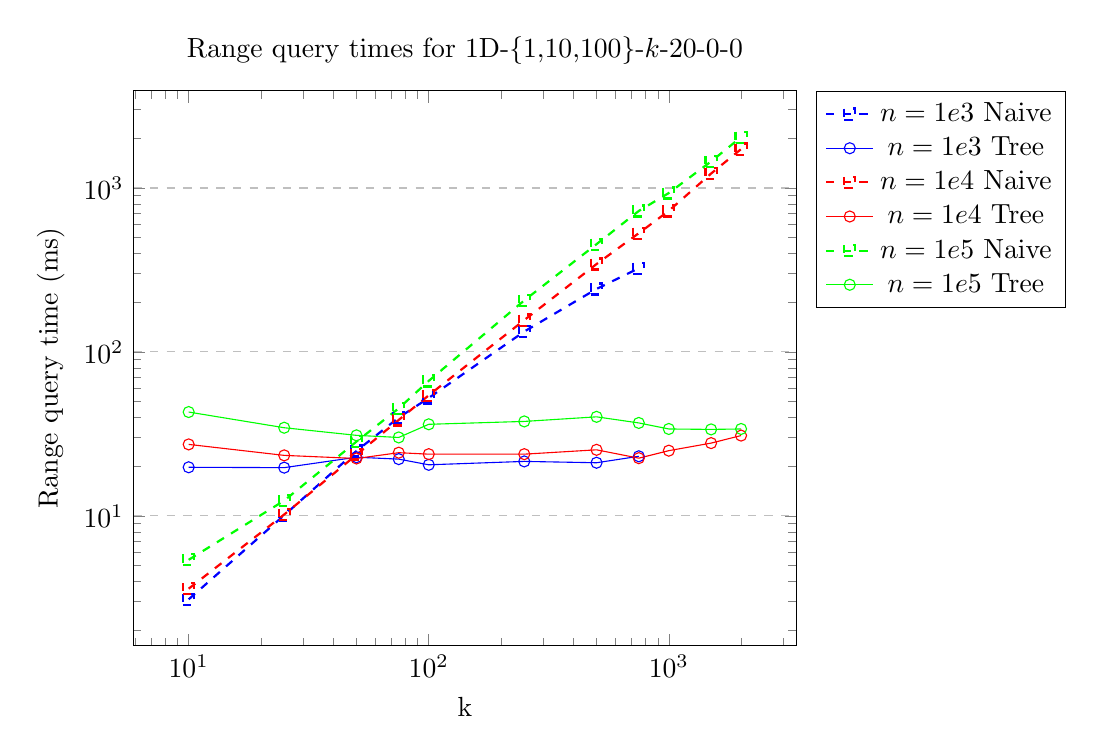
\begin{tikzpicture}
    \begin{axis}[
        title={Range query times for 1D-\{1,10,100\}-$k$-20-0-0},
        xmode=log,
        ymode=log,
        xlabel={k},
        ylabel={Range query time (ms)},
        legend pos=outer north east,
        ymajorgrids=true,
        grid style=dashed,
    ]
    \addplot[
        color=blue,
        mark=square,
        dashed, thick,
        ]
        coordinates {
            (10, 3.1)
            (25, 10.1)
            (50, 24.9)
            (75, 39.8)
            (100, 52.4)
            (250, 133.2)
            (500, 242.2)
            (750, 324.0)
        };
    \addlegendentry{$n=1e3$ Naive}
    \addplot[
        color=blue,
        mark=o,
        ]
        coordinates {
            (10, 19.8)
            (25, 19.7)
            (50, 22.8)
            (75, 22.2)
            (100, 20.5)
            (250, 21.5)
            (500, 21.1)
            (750, 23.1)
        };
    \addlegendentry{$n=1e3$ Tree}
    
    \addplot[
        color=red,
        mark=square,
        dashed, thick
        ]
        coordinates {
            (10, 3.6)
            (25, 10.2)
            (50, 23.6)
            (75, 38.5)
            (100, 54.4)
            (250, 156.4)
            (500, 343.5)
            (750, 530.0)
            (1000, 725.0)
            (1500, 1224.4)
            (2000, 1725.3)
        };
    \addlegendentry{$n=1e4$ Naive}
    \addplot[
        color=red,
        mark=o,
        ]
        coordinates {
        (10, 27.3)
        (25, 23.4)
        (50, 22.4)
        (75, 24.3)
        (100, 23.8)
        (250, 23.8)
        (500, 25.3)
        (750, 22.5)
        (1000, 25.0)
        (1500, 27.8)
        (2000, 30.9)
        };
    \addlegendentry{$n=1e4$ Tree}
    
    \addplot[
        color=green,
        mark=square,
        dashed, thick,
        ]
        coordinates {
            (10, 5.4)
            (25, 12.4)
            (50, 28.4)
            (75, 45.3)
            (100, 66.6)
            (250, 206.2)
            (500, 454.2)
            (750, 724.1)
            (1000, 931.0)
            (1500, 1450.9)
            (2000, 2040.4)
        };
    \addlegendentry{$n=1e5$ Naive}
    \addplot[
        color=green,
        mark=o,
        ]
        coordinates {
            (10, 43.0)
            (25, 34.5)
            (50, 31.0)
            (75, 30.1)
            (100, 36.2)
            (250, 37.7)
            (500, 40.2)
            (750, 36.9)
            (1000, 33.9)
            (1500, 33.7)
            (2000, 33.9)
        };
    \addlegendentry{$n=1e5$ Tree}
    \end{axis}
\end{tikzpicture}
}
\resizebox{8cm}{!}{
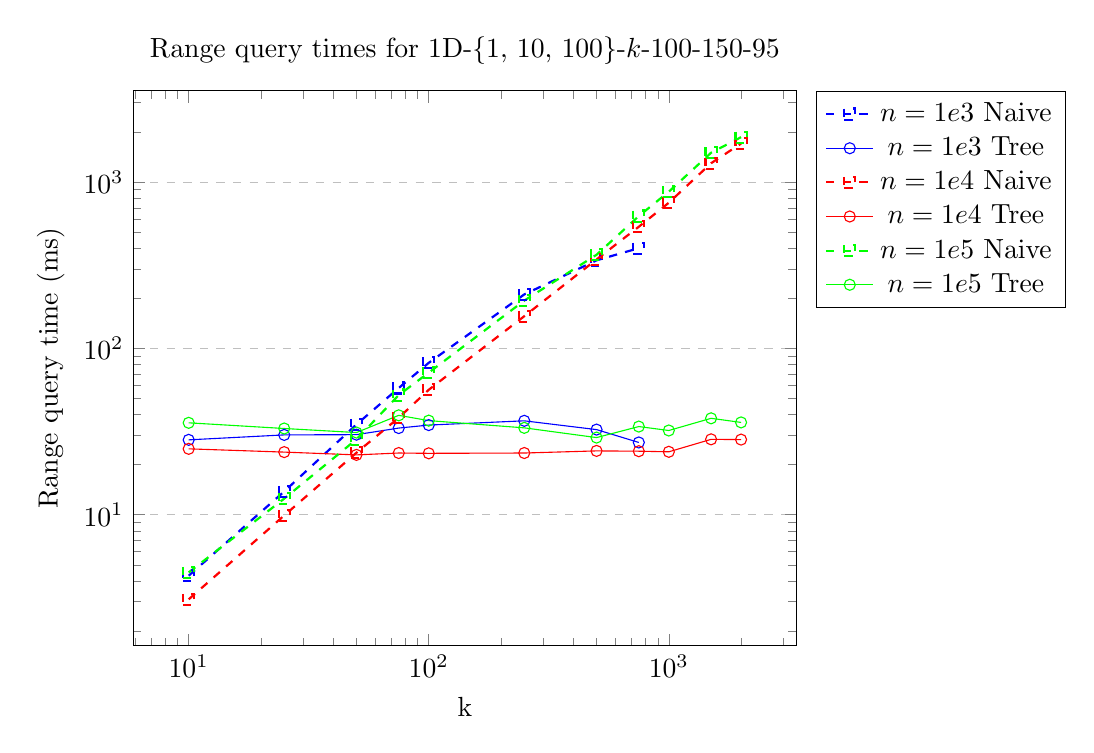
\begin{tikzpicture}
    \begin{axis}[
        title={Range query times for 1D-\{1, 10, 100\}-$k$-100-150-95 },
        xmode=log,
        ymode=log,
        xlabel={k},
        ylabel={Range query time (ms)},
        legend pos=outer north east,
        ymajorgrids=true,
        grid style=dashed,
    ]
    \addplot[
        color=blue,
        mark=square,
        dashed, thick,
        ]
        coordinates {
            (10, 4.3)
            (25, 13.8)
            (50, 34.9)
            (75, 57.8)
            (100, 81.9)
            (250, 211.2)
            (500, 338.5)
            (750, 400.6)
        };
    \addlegendentry{$n=1e3$ Naive}
    \addplot[
        color=blue,
        mark=o,
        ]
        coordinates {
            (10, 28.2)
            (25, 30.2)
            (50, 30.3)
            (75, 33.2)
            (100, 34.6)
            (250, 36.7)
            (500, 32.5)
            (750, 27.2)
        };
    \addlegendentry{$n=1e3$ Tree}
    
    \addplot[
        color=red,
        mark=square,
        dashed, thick
        ]
        coordinates {
            (10, 3.1)
            (25, 9.9)
            (50, 23.6)
            (75, 38.3)
            (100, 56.4)
            (250, 156.2)
            (500, 342.6)
            (750, 539.0)
            (1000, 751.2)
            (1500, 1298.7) 
(2000, 1704.1) 
        };
    \addlegendentry{$n=1e4$ Naive}
    \addplot[
        color=red,
        mark=o,
        ]
        coordinates {
            (10, 24.9)
            (25, 23.8)
            (50, 22.9)
            (75, 23.5)
            (100, 23.4)
            (250, 23.5)
            (500, 24.2)
            (750, 24.1)
            (1000, 23.9)
            (1500, 28.4)
(2000, 28.3)
        };
    \addlegendentry{$n=1e4$ Tree}
    
    \addplot[
        color=green,
        mark=square,
        dashed, thick,
        ]
        coordinates {
            (10, 4.5)
            (25, 12.5)
            (50, 28.4)
            (75, 52.4)
            (100, 71.5)
            (250, 193.9)
            (500, 365.6)
            (750, 624.7)
            (1000, 875.4)
            (1500, 1501.1)
(2000, 1862.5)
        };
    \addlegendentry{$n=1e5$ Naive}
    \addplot[
        color=green,
        mark=o,
        ]
        coordinates {
            (10, 35.7)
            (25, 33.0)
            (50, 31.2)
            (75, 39.6)
            (100, 36.8)
            (250, 33.3)
            (500, 29.1)
            (750, 33.9)
            (1000, 32.1)
            (1500, 38.0)
(2000, 35.9)
        };
    \addlegendentry{$n=1e5$ Tree}
    \end{axis}
    \end{tikzpicture}
}

% B1, B2, C1, C2
\hskip-2cm
\resizebox{8cm}{!}{
    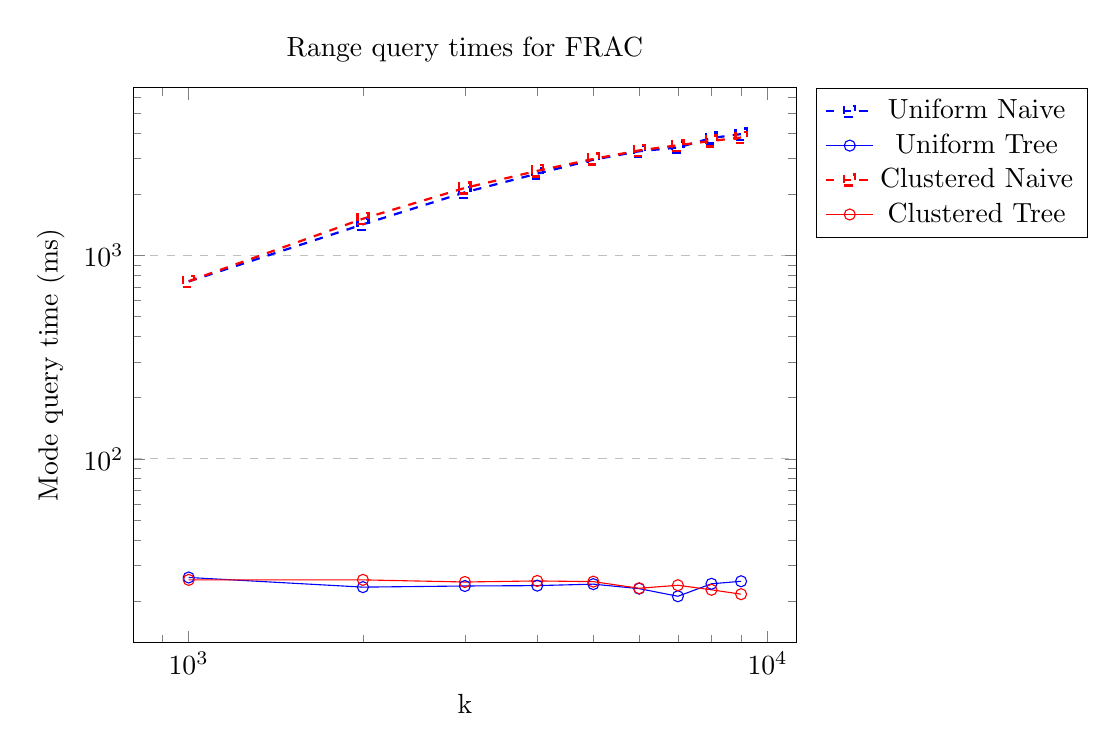
\begin{tikzpicture}
    \begin{axis}[
        title={Range query times for FRAC},
        xmode=log,
        ymode=log,
        xlabel={k},
        ylabel={Mode query time (ms)},
        legend pos=outer north east,
        ymajorgrids=true,
        grid style=dashed,
    ]
    \addplot[
        color=blue,
        mark=square,
        dashed, thick,
        ]
        coordinates {
            (1000, 746.1)
            (2000, 1423.7)
            (3000, 2046.1)
            (4000, 2529.4)
            (5000, 2960.1)
            (6000, 3258.7)
            (7000, 3399.4)
            (8000, 3785.1)
            (9000, 3958.8)
        };
    \addlegendentry{Uniform Naive}
    \addplot[
        color=blue,
        mark=o,
        ]
        coordinates {
            (1000, 26.1)
            (2000, 23.4)
            (3000, 23.7)
            (4000, 23.8)
            (5000, 24.2)
            (6000, 23.0)
            (7000, 21.1)
            (8000, 24.3)
            (9000, 25.0)
        };
    \addlegendentry{Uniform Tree}
    
    \addplot[
        color=red,
        mark=square,
        dashed, thick
        ]
        coordinates {
            (1000, 748.2)
            (2000, 1517.7)
            (3000, 2151.0)
            (4000, 2609.7)
            (5000, 2986.5)
            (6000, 3289.9)
            (7000, 3489.2)
            (8000, 3661.8)
            (9000, 3808.8)
        };
    \addlegendentry{Clustered Naive}
    \addplot[
        color=red,
        mark=o,
        ]
        coordinates {
            (1000, 25.4)
            (2000, 25.4)
            (3000, 24.8)
            (4000, 25.1)
            (5000, 24.9)
            (6000, 23.1)
            (7000, 23.9)
            (8000, 22.7)
            (9000, 21.6)
        };
    \addlegendentry{Clustered Tree}
    \end{axis}
    \end{tikzpicture}
}
\resizebox{8cm}{!}{
    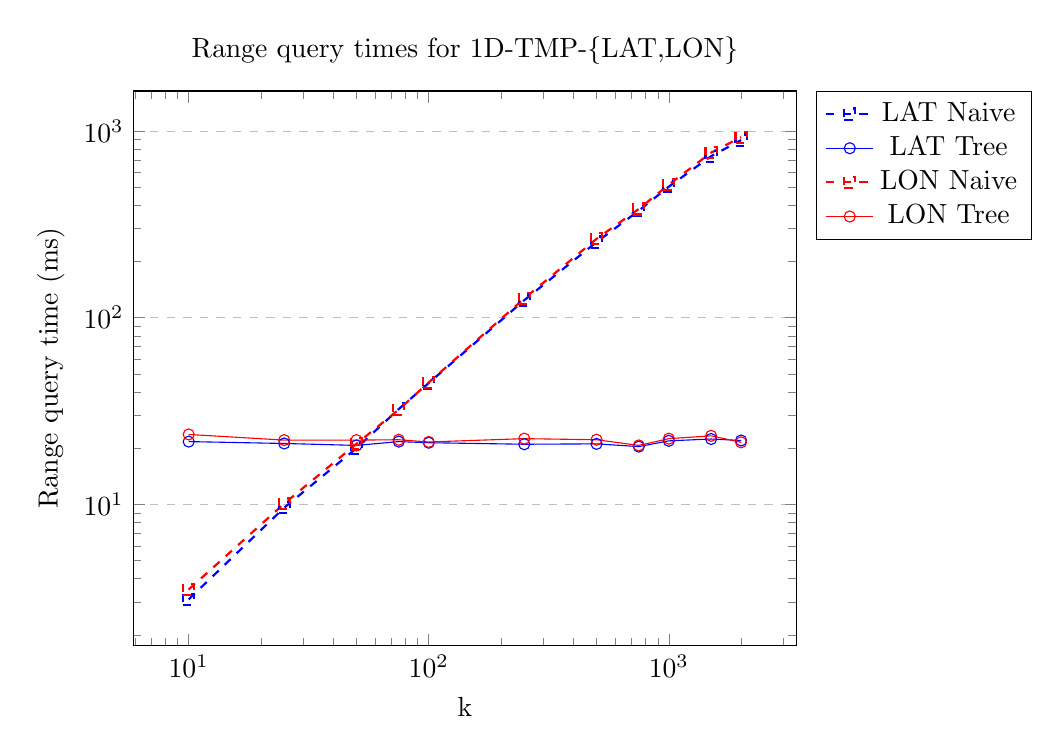
\begin{tikzpicture}
    \begin{axis}[
        title={Range query times for 1D-TMP-\{LAT,LON\}},
        xmode=log,
        ymode=log,
        xlabel={k},
        ylabel={Range query time (ms)},
        legend pos=outer north east,
        ymajorgrids=true,
        grid style=dashed,
    ]
    \addplot[
        color=blue,
        mark=square,
        dashed, thick,
        ]
        coordinates {
            (10, 3.1)
            (25, 9.6)
            (50, 20.0)
            (75, 32.4)
            (100, 44.7)
            (250, 124.1)
            (500, 254.2)
            (750, 374.5)
            (1000, 503.8)
            (1500, 733.0)
(2000, 894.4)
        };
    \addlegendentry{LAT Naive}
    \addplot[
        color=blue,
        mark=o,
        ]
        coordinates {
            (10, 21.7)
            (25, 21.2)
            (50, 20.7)
            (75, 21.7)
            (100, 21.4)
            (250, 21.0)
            (500, 21.1)
            (750, 20.4)
            (1000, 21.9)
            (1500, 22.4)
(2000, 22.0)
        };
    \addlegendentry{LAT Tree}
    
    \addplot[
        color=red,
        mark=square,
        dashed, thick
        ]
        coordinates {
            (10, 3.5)
            (25, 10.1)
            (50, 21.1)
            (75, 32.2)
            (100, 45.0)
            (250, 126.8)
            (500, 264.6)
            (750, 382.6)
            (1000, 516.3)
            (1500, 766.4)
(2000, 927.4)
        };
    \addlegendentry{LON Naive}
    \addplot[
        color=red,
        mark=o,
        ]
        coordinates {
            (10, 23.7)
            (25, 22.1)
            (50, 22.1)
            (75, 22.2)
            (100, 21.6)
            (250, 22.5)
            (500, 22.2)
            (750, 20.7)
            (1000, 22.5)
            (1500, 23.3)
(2000, 21.5)
        };
    \addlegendentry{LON Tree}
    \end{axis}
    \end{tikzpicture}
}

% All data
% \hskip-2cm
% \resizebox{8cm}{!}{
%     \begin{tikzpicture}
%     \begin{axis}[
%         title={Range query times for A1-A3},
%         xmode=log,
%         ymode=log,
%         xlabel={k},
%         ylabel={Range query time (ms)},
%         legend pos=outer north east,
%         ymajorgrids=true,
%         grid style=dashed,
%     ]
%     \addplot[
%         color=blue,
%         mark=square,
%         dashed, thick,
%         ]
%         coordinates {
%             (10, 3.1)
%             (25, 10.1)
%             (50, 24.9)
%             (75, 39.8)
%             (100, 52.4)
%             (250, 133.2)
%             (500, 242.2)
%             (750, 324.0)
%         };
%     \addlegendentry{A1 Naive}
%     \addplot[
%         color=blue,
%         mark=o,
%         ]
%         coordinates {
%             (10, 19.8)
%             (25, 19.7)
%             (50, 22.8)
%             (75, 22.2)
%             (100, 20.5)
%             (250, 21.5)
%             (500, 21.1)
%             (750, 23.1)
%         };
%     \addlegendentry{A1 Tree}
    
%     \addplot[
%         color=red,
%         mark=square,
%         dashed, thick
%         ]
%         coordinates {
%             (10, 3.6)
%             (25, 10.2)
%             (50, 23.6)
%             (75, 38.5)
%             (100, 54.4)
%             (250, 156.4)
%             (500, 343.5)
%             (750, 530.0)
%             (1000, 725.0)
%             (1500, 1224.4)
%             (2000, 1725.3)
%         };
%     \addlegendentry{A2 Naive}
%     \addplot[
%         color=red,
%         mark=o,
%         ]
%         coordinates {
%         (10, 27.3)
%         (25, 23.4)
%         (50, 22.4)
%         (75, 24.3)
%         (100, 23.8)
%         (250, 23.8)
%         (500, 25.3)
%         (750, 22.5)
%         (1000, 25.0)
%         (1500, 27.8)
%         (2000, 30.9)
%         };
%     \addlegendentry{A2 Tree}
    
%     \addplot[
%         color=green,
%         mark=square,
%         dashed, thick,
%         ]
%         coordinates {
%             (10, 5.4)
%             (25, 12.4)
%             (50, 28.4)
%             (75, 45.3)
%             (100, 66.6)
%             (250, 206.2)
%             (500, 454.2)
%             (750, 724.1)
%             (1000, 931.0)
%             (1500, 1450.9)
%             (2000, 2040.4)
%         };
%     \addlegendentry{A3 Naive}
%     \addplot[
%         color=green,
%         mark=o,
%         ]
%         coordinates {
%             (10, 43.0)
%             (25, 34.5)
%             (50, 31.0)
%             (75, 30.1)
%             (100, 36.2)
%             (250, 37.7)
%             (500, 40.2)
%             (750, 36.9)
%             (1000, 33.9)
%             (1500, 33.7)
%             (2000, 33.9)
%         };
%     \addlegendentry{A3 Tree}
%     \end{axis}
%     \end{tikzpicture}
% }
% \resizebox{8cm}{!}{
%     \begin{tikzpicture}
%     \begin{axis}[
%         title={Range query times for A4-A6},
%         xmode=log,
%         ymode=log,
%         xlabel={k},
%         ylabel={Range query time (ms)},
%         legend pos=outer north east,
%         ymajorgrids=true,
%         grid style=dashed,
%     ]
%     \addplot[
%         color=blue,
%         mark=square,
%         dashed, thick,
%         ]
%         coordinates {
%             (10, 3.5)
%             (25, 10.8)
%             (50, 24.8)
%             (75, 39.2)
%             (100, 58.2)
%             (250, 153.0)
%             (500, 290.8)
%             (750, 349.7)
%         };
%     \addlegendentry{A4 Naive}
%     \addplot[
%         color=blue,
%         mark=o,
%         ]
%         coordinates {
%             (10, 21.3)
%             (25, 21.7)
%             (50, 20.9)
%             (75, 21.6)
%             (100, 22.1)
%             (250, 26.6)
%             (500, 24.8)
%             (750, 24.4)
%         };
%     \addlegendentry{A4 Tree}
    
%     \addplot[
%         color=red,
%         mark=square,
%         dashed, thick
%         ]
%         coordinates {
%             (10, 3.3)
%             (25, 10.2)
%             (50, 23.6)
%             (75, 38.5)
%             (100, 54.9)
%             (250, 159.0)
%             (500, 345.1)
%             (750, 529.8)
%             (1000, 720.5)
%             (1500, 1271.0)
% (2000, 1713.8)
%         };
%     \addlegendentry{A5 Naive}
%     \addplot[
%         color=red,
%         mark=o,
%         ]
%         coordinates {
%             (10, 24.0)
%             (25, 23.0)
%             (50, 24.7)
%             (75, 22.4)
%             (100, 22.6)
%             (250, 24.1)
%             (500, 23.8)
%             (750, 23.0)
%             (1000, 22.7)
%             (1500, 28.3)
% (2000, 26.6)
%         };
%     \addlegendentry{A5 Tree}
    
%     \addplot[
%         color=green,
%         mark=square,
%         dashed, thick,
%         ]
%         coordinates {
%             (10, 4.5)
%             (25, 12.7)
%             (50, 28.3)
%             (75, 46.6)
%             (100, 66.3)
%             (250, 214.9)
%             (500, 445.1)
%             (750, 676.8)
%             (1000, 892.6)
%             (1500, 1448.5)
% (2000, 2074.2)
%         };
%     \addlegendentry{A6 Naive}
%     \addplot[
%         color=green,
%         mark=o,
%         ]
%         coordinates {
%             (10, 39.1)
%             (25, 35.2)
%             (50, 33.4)
%             (75, 30.9)
%             (100, 32.9)
%             (250, 37.8)
%             (500, 36.9)
%             (750, 32.5)
%             (1000, 33.1)
%             (1500, 33.5)
% (2000, 33.5)
%         };
%     \addlegendentry{A6 Tree}
%     \end{axis}
%     \end{tikzpicture}
% }

% % A7-A12
% \hskip-2cm
% \resizebox{8cm}{!}{
%     \begin{tikzpicture}
%     \begin{axis}[
%         title={Range query times for A7-A9},
%         xmode=log,
%         ymode=log,
%         xlabel={k},
%         ylabel={Range query time (ms)},
%         legend pos=outer north east,
%         ymajorgrids=true,
%         grid style=dashed,
%     ]
%     \addplot[
%         color=blue,
%         mark=square,
%         dashed, thick,
%         ]
%         coordinates {
%             (10, 3.8)
%             (25, 12.8)
%             (50, 32.4)
%             (75, 48.2)
%             (100, 65.0)
%             (250, 170.4)
%             (500, 301.1)
%             (750, 420.0)
%         };
%     \addlegendentry{A7 Naive}
%     \addplot[
%         color=blue,
%         mark=o,
%         ]
%         coordinates {
%             (10, 26.4)
%             (25, 27.8)
%             (50, 29.6)
%             (75, 26.7)
%             (100, 28.5)
%             (250, 31.4)
%             (500, 28.4)
%             (750, 34.8)
%         };
%     \addlegendentry{A7 Tree}
    
%     \addplot[
%         color=red,
%         mark=square,
%         dashed, thick
%         ]
%         coordinates {
%             (10, 3.4)
%             (25, 10.0)
%             (50, 23.5)
%             (75, 39.5)
%             (100, 55.6)
%             (250, 166.0)
%             (500, 348.6)
%             (750, 536.6)
%             (1000, 717.6)
%             (1500, 1317.7)
% (2000, 1691.2)
%         };
%     \addlegendentry{A8 Naive}
%     \addplot[
%         color=red,
%         mark=o,
%         ]
%         coordinates {
%             (10, 23.2)
%             (25, 21.9)
%             (50, 21.8)
%             (75, 24.2)
%             (100, 22.7)
%             (250, 25.3)
%             (500, 26.1)
%             (750, 24.3)
%             (1000, 23.0)
%             (1500, 27.4)
% (2000, 26.6)
%         };
%     \addlegendentry{A8 Tree}
    
%     \addplot[
%         color=green,
%         mark=square,
%         dashed, thick,
%         ]
%         coordinates {
%             (10, 4.6)
%             (25, 11.8)
%             (50, 27.3)
%             (75, 52.9)
%             (100, 68.9)
%             (250, 191.9)
%             (500, 368.1)
%             (750, 618.4)
%             (1000, 862.7)
%             (1500, 1474.6)
% (2000, 1880.3)
%         };
%     \addlegendentry{A9 Naive}
%     \addplot[
%         color=green,
%         mark=o,
%         ]
%         coordinates {
%             (10, 34.7)
%             (25, 31.7)
%             (50, 33.1)
%             (75, 33.7)
%             (100, 33.5)
%             (250, 33.4)
%             (500, 28.1)
%             (750, 31.2)
%             (1000, 31.5)
%             (1500, 39.5)
% (2000, 31.8)
%         };
%     \addlegendentry{A9 Tree}
%     \end{axis}
%     \end{tikzpicture}
% }
% \resizebox{8cm}{!}{
%     \begin{tikzpicture}
%     \begin{axis}[
%         title={Range query times for A10-A12},
%         xmode=log,
%         ymode=log,
%         xlabel={k},
%         ylabel={Range query time (ms)},
%         legend pos=outer north east,
%         ymajorgrids=true,
%         grid style=dashed,
%     ]
%     \addplot[
%         color=blue,
%         mark=square,
%         dashed, thick,
%         ]
%         coordinates {
%             (10, 4.3)
%             (25, 13.8)
%             (50, 34.9)
%             (75, 57.8)
%             (100, 81.9)
%             (250, 211.2)
%             (500, 338.5)
%             (750, 400.6)
%         };
%     \addlegendentry{A10 Naive}
%     \addplot[
%         color=blue,
%         mark=o,
%         ]
%         coordinates {
%             (10, 28.2)
%             (25, 30.2)
%             (50, 30.3)
%             (75, 33.2)
%             (100, 34.6)
%             (250, 36.7)
%             (500, 32.5)
%             (750, 27.2)
%         };
%     \addlegendentry{A10 Tree}
    
%     \addplot[
%         color=red,
%         mark=square,
%         dashed, thick
%         ]
%         coordinates {
%             (10, 3.1)
%             (25, 9.9)
%             (50, 23.6)
%             (75, 38.3)
%             (100, 56.4)
%             (250, 156.2)
%             (500, 342.6)
%             (750, 539.0)
%             (1000, 751.2)
%             (1500, 1298.7) 
% (2000, 1704.1) 
%         };
%     \addlegendentry{A11 Naive}
%     \addplot[
%         color=red,
%         mark=o,
%         ]
%         coordinates {
%             (10, 24.9)
%             (25, 23.8)
%             (50, 22.9)
%             (75, 23.5)
%             (100, 23.4)
%             (250, 23.5)
%             (500, 24.2)
%             (750, 24.1)
%             (1000, 23.9)
%             (1500, 28.4)
% (2000, 28.3)
%         };
%     \addlegendentry{A11 Tree}
    
%     \addplot[
%         color=green,
%         mark=square,
%         dashed, thick,
%         ]
%         coordinates {
%             (10, 4.5)
%             (25, 12.5)
%             (50, 28.4)
%             (75, 52.4)
%             (100, 71.5)
%             (250, 193.9)
%             (500, 365.6)
%             (750, 624.7)
%             (1000, 875.4)
%             (1500, 1501.1)
% (2000, 1862.5)
%         };
%     \addlegendentry{A12 Naive}
%     \addplot[
%         color=green,
%         mark=o,
%         ]
%         coordinates {
%             (10, 35.7)
%             (25, 33.0)
%             (50, 31.2)
%             (75, 39.6)
%             (100, 36.8)
%             (250, 33.3)
%             (500, 29.1)
%             (750, 33.9)
%             (1000, 32.1)
%             (1500, 38.0)
% (2000, 35.9)
%         };
%     \addlegendentry{A12 Tree}
%     \end{axis}
%     \end{tikzpicture}
% }

% % B1, B2, C1, C2
% \hskip-2cm
% \resizebox{8cm}{!}{
%     \begin{tikzpicture}
%     \begin{axis}[
%         title={Range query times for B1 and B2},
%         xmode=log,
%         ymode=log,
%         xlabel={k},
%         ylabel={Mode query time (ms)},
%         legend pos=outer north east,
%         ymajorgrids=true,
%         grid style=dashed,
%     ]
%     \addplot[
%         color=blue,
%         mark=square,
%         dashed, thick,
%         ]
%         coordinates {
%             (1000, 746.1)
%             (2000, 1423.7)
%             (3000, 2046.1)
%             (4000, 2529.4)
%             (5000, 2960.1)
%             (6000, 3258.7)
%             (7000, 3399.4)
%             (8000, 3785.1)
%             (9000, 3958.8)
%         };
%     \addlegendentry{B1 Naive}
%     \addplot[
%         color=blue,
%         mark=o,
%         ]
%         coordinates {
%             (1000, 26.1)
%             (2000, 23.4)
%             (3000, 23.7)
%             (4000, 23.8)
%             (5000, 24.2)
%             (6000, 23.0)
%             (7000, 21.1)
%             (8000, 24.3)
%             (9000, 25.0)
%         };
%     \addlegendentry{B1 Tree}
    
%     \addplot[
%         color=red,
%         mark=square,
%         dashed, thick
%         ]
%         coordinates {
%             (1000, 748.2)
%             (2000, 1517.7)
%             (3000, 2151.0)
%             (4000, 2609.7)
%             (5000, 2986.5)
%             (6000, 3289.9)
%             (7000, 3489.2)
%             (8000, 3661.8)
%             (9000, 3808.8)
%         };
%     \addlegendentry{B2 Naive}
%     \addplot[
%         color=red,
%         mark=o,
%         ]
%         coordinates {
%             (1000, 25.4)
%             (2000, 25.4)
%             (3000, 24.8)
%             (4000, 25.1)
%             (5000, 24.9)
%             (6000, 23.1)
%             (7000, 23.9)
%             (8000, 22.7)
%             (9000, 21.6)
%         };
%     \addlegendentry{B2 Tree}
%     \end{axis}
%     \end{tikzpicture}
% }
% \resizebox{8cm}{!}{
%     \begin{tikzpicture}
%     \begin{axis}[
%         title={Range query times for C1 and C2},
%         xmode=log,
%         ymode=log,
%         xlabel={k},
%         ylabel={Range query time (ms)},
%         legend pos=outer north east,
%         ymajorgrids=true,
%         grid style=dashed,
%     ]
%     \addplot[
%         color=blue,
%         mark=square,
%         dashed, thick,
%         ]
%         coordinates {
%             (10, 3.1)
%             (25, 9.6)
%             (50, 20.0)
%             (75, 32.4)
%             (100, 44.7)
%             (250, 124.1)
%             (500, 254.2)
%             (750, 374.5)
%             (1000, 503.8)
%             (1500, 733.0)
% (2000, 894.4)
%         };
%     \addlegendentry{C1 Naive}
%     \addplot[
%         color=blue,
%         mark=o,
%         ]
%         coordinates {
%             (10, 21.7)
%             (25, 21.2)
%             (50, 20.7)
%             (75, 21.7)
%             (100, 21.4)
%             (250, 21.0)
%             (500, 21.1)
%             (750, 20.4)
%             (1000, 21.9)
%             (1500, 22.4)
% (2000, 22.0)
%         };
%     \addlegendentry{C1 Tree}
    
%     \addplot[
%         color=red,
%         mark=square,
%         dashed, thick
%         ]
%         coordinates {
%             (10, 3.5)
%             (25, 10.1)
%             (50, 21.1)
%             (75, 32.2)
%             (100, 45.0)
%             (250, 126.8)
%             (500, 264.6)
%             (750, 382.6)
%             (1000, 516.3)
%             (1500, 766.4)
% (2000, 927.4)
%         };
%     \addlegendentry{C2 Naive}
%     \addplot[
%         color=red,
%         mark=o,
%         ]
%         coordinates {
%             (10, 23.7)
%             (25, 22.1)
%             (50, 22.1)
%             (75, 22.2)
%             (100, 21.6)
%             (250, 22.5)
%             (500, 22.2)
%             (750, 20.7)
%             (1000, 22.5)
%             (1500, 23.3)
% (2000, 21.5)
%         };
%     \addlegendentry{C2 Tree}
%     \end{axis}
%     \end{tikzpicture}
% }

% A1-A6
\hskip-2cm
\resizebox{8cm}{!}{
    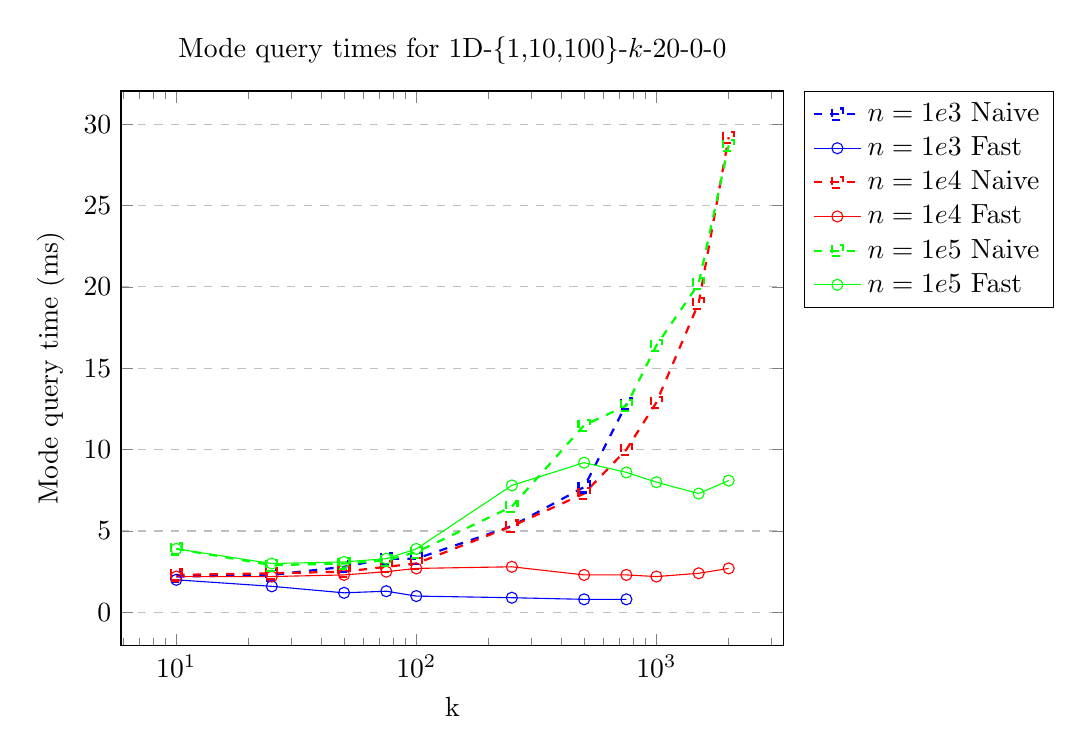
\begin{tikzpicture}
    \begin{axis}[
        title={Mode query times for 1D-\{1,10,100\}-$k$-20-0-0},
        xlabel={k},xmode=log,
        ylabel={Mode query time (ms)},
        legend pos=outer north east,
        ymajorgrids=true,
        grid style=dashed,
        legend cell align={left}
    ]
    \addplot[
        color=blue,
        mark=square,
        dashed, thick,
        ]
        coordinates {
            (10, 2.2)
            (25, 2.3)
            (50, 2.8)
            (75, 3.3)
            (100, 3.3)
            (250, 5.3)
            (500, 7.7)
            (750, 12.8)
        };
    \addlegendentry{$n=1e3$ Naive}
    \addplot[
        color=blue,
        mark=o,
        ]
        coordinates {
            (10, 2.0)
            (25, 1.6)
            (50, 1.2)
            (75, 1.3)
            (100, 1.0)
            (250, 0.9)
            (500, 0.8)
            (750, 0.8)
        };
    \addlegendentry{$n=1e3$ Fast}
    
    \addplot[
        color=red,
        mark=square,
        dashed, thick
        ]
        coordinates {
            (10, 2.3)
            (25, 2.4)
            (50, 2.5)
            (75, 2.8)
            (100, 3.0)
            (250, 5.3)
            (500, 7.3)
            (750, 10.0)
            (1000, 12.9)
            (1500, 19.0)
            (2000, 29.2)
        };
    \addlegendentry{$n=1e4$ Naive}
    \addplot[
        color=red,
        mark=o,
        ]
        coordinates {
            (10, 2.2)
            (25, 2.2)
            (50, 2.3)
            (75, 2.5)
            (100, 2.7)
            (250, 2.8)
            (500, 2.3)
            (750, 2.3)
            (1000, 2.2)
            (1500, 2.4)
            (2000, 2.7)
        };
    \addlegendentry{$n=1e4$ Fast}
    
    \addplot[
        color=green,
        mark=square,
        dashed, thick,
        ]
        coordinates {
            (10, 3.9)
            (25, 2.9)
            (50, 3.0)
            (75, 3.2)
            (100, 3.7)
            (250, 6.5)
            (500, 11.5)
            (750, 12.7)
            (1000, 16.4)
            (1500, 20.2)
(2000, 28.7)
        };
    \addlegendentry{$n=1e5$ Naive}
    \addplot[
        color=green,
        mark=o,
        ]
        coordinates {
            (10, 3.9)
            (25, 3.0)
            (50, 3.1)
            (75, 3.3)
            (100, 3.9)
            (250, 7.8)
            (500, 9.2)
            (750, 8.6)
            (1000, 8.0)
            (1500, 7.3) 
(2000, 8.1) 
        };
    \addlegendentry{$n=1e5$ Fast}
    \end{axis}
    \end{tikzpicture}
}
\resizebox{8cm}{!}{
    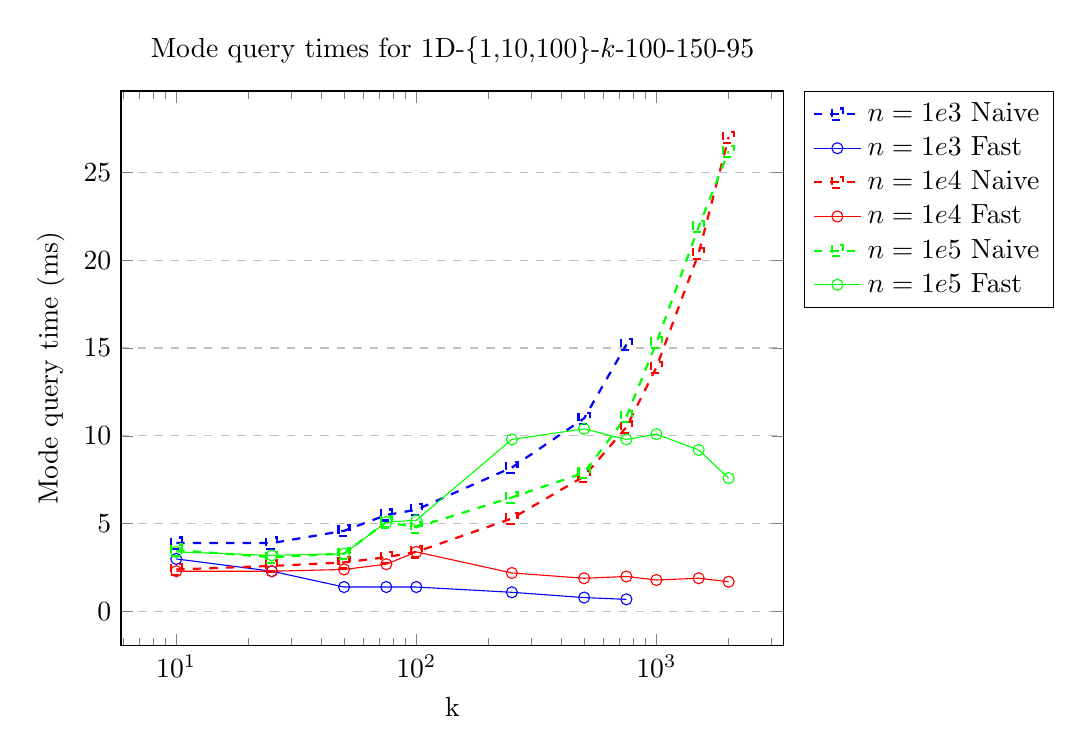
\begin{tikzpicture}
    \begin{axis}[
        title={Mode query times for 1D-\{1,10,100\}-$k$-100-150-95 },
        xlabel={k},xmode=log,
        ylabel={Mode query time (ms)},
        legend pos=outer north east,
        ymajorgrids=true,
        grid style=dashed,
        legend cell align={left}
    ]
    \addplot[
        color=blue,
        mark=square,
        dashed, thick,
        ]
        coordinates {
            (10, 3.9)
            (25, 3.9)
            (50, 4.6)
            (75, 5.5)
            (100, 5.8)
            (250, 8.2)
            (500, 11.0)
            (750, 15.2)
        };
    \addlegendentry{$n=1e3$ Naive}
    \addplot[
        color=blue,
        mark=o,
        ]
        coordinates {
            (10, 3.0)
            (25, 2.3)
            (50, 1.4)
            (75, 1.4)
            (100, 1.4)
            (250, 1.1)
            (500, 0.8)
            (750, 0.7)
        };
    \addlegendentry{$n=1e3$ Fast}
    
    \addplot[
        color=red,
        mark=square,
        dashed, thick
        ]
        coordinates {
            (10, 2.4)
            (25, 2.6)
            (50, 2.8)
            (75, 3.1)
            (100, 3.4)
            (250, 5.3)
            (500, 7.7)
            (750, 10.5)
            (1000, 13.9)
            (1500, 20.4)
(2000, 27.0)
        };
    \addlegendentry{$n=1e4$ Naive}
    \addplot[
        color=red,
        mark=o,
        ]
        coordinates {
           (10, 2.3)
            (25, 2.3)
            (50, 2.4)
            (75, 2.7)
            (100, 3.4)
            (250, 2.2)
            (500, 1.9)
            (750, 2.0)
            (1000, 1.8)
            (1500, 1.9) 
(2000, 1.7) 
        };
    \addlegendentry{$n=1e4$ Fast}
    
    \addplot[
        color=green,
        mark=square,
        dashed, thick,
        ]
        coordinates {
            (10, 3.5)
            (25, 3.1)
            (50, 3.3)
            (75, 5.1)
            (100, 4.8)
            (250, 6.5)
            (500, 7.9)
            (750, 11.1)
            (1000, 15.3)
            (1500, 21.9)
(2000, 26.2)
        };
    \addlegendentry{$n=1e5$ Naive}
    \addplot[
        color=green,
        mark=o,
        ]
        coordinates {
            (10, 3.4)
            (25, 3.2)
            (50, 3.3)
            (75, 5.1)
            (100, 5.2)
            (250, 9.8)
            (500, 10.4)
            (750, 9.8)
            (1000, 10.1)
            (1500, 9.2) 
(2000, 7.6) 
        };
    \addlegendentry{$n=1e5$ Fast}
    \end{axis}
    \end{tikzpicture}
}

% B1, B2, C1, C2
\hskip-2cm
\resizebox{8cm}{!}{
    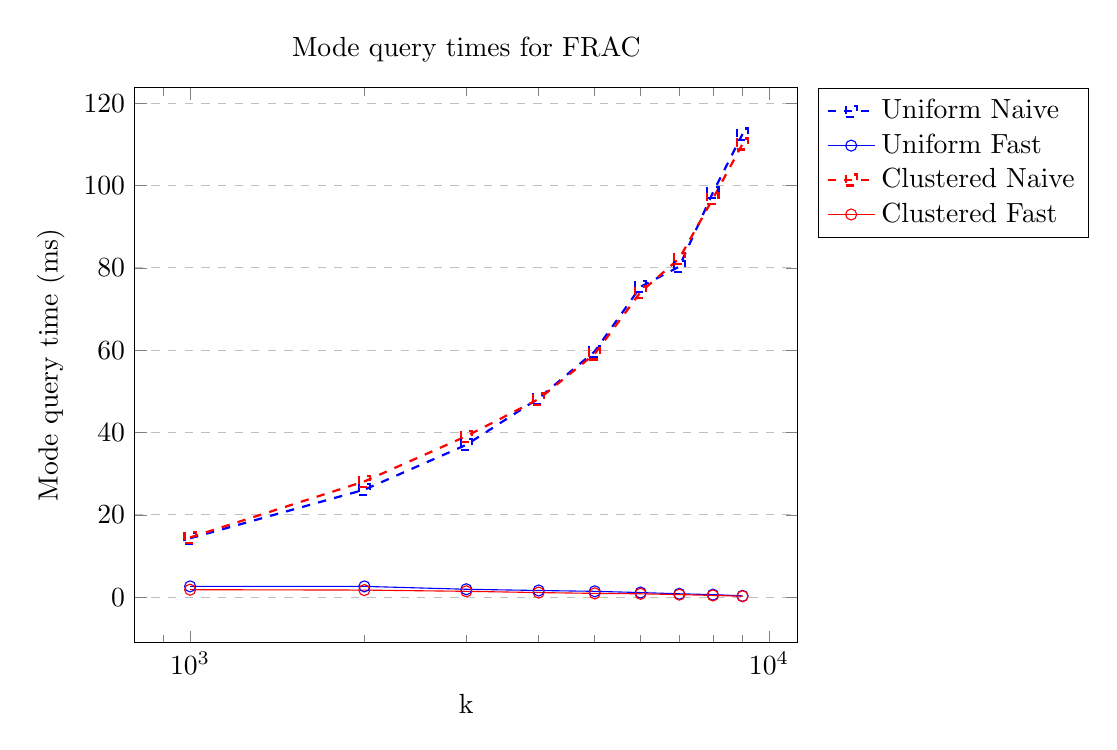
\begin{tikzpicture}
    \begin{axis}[
        title={Mode query times for FRAC},
        xlabel={k},xmode=log,
        ylabel={Mode query time (ms)},
        legend pos=outer north east,
        ymajorgrids=true,
        grid style=dashed,
        legend cell align={left}
    ]
    \addplot[
        color=blue,
        mark=square,
        dashed, thick,
        ]
        coordinates {
            (1000, 14.3)
            (2000, 26.1)
            (3000, 37.0)
            (4000, 48.3)
            (5000, 59.7)
            (6000, 75.4)
            (7000, 80.3)
            (8000, 98.3)
            (9000, 112.5)
        };
    \addlegendentry{Uniform Naive}
    \addplot[
        color=blue,
        mark=o,
        ]
        coordinates {
            (1000, 2.6)
            (2000, 2.6)
            (3000, 1.9)
            (4000, 1.6)
            (5000, 1.4)
            (6000, 1.1)
            (7000, 0.8)
            (8000, 0.6)
            (9000, 0.3)
        };
    \addlegendentry{Uniform Fast}
    
    \addplot[
        color=red,
        mark=square,
        dashed, thick
        ]
        coordinates {
            (1000, 14.5)
            (2000, 28.1)
            (3000, 39.1)
            (4000, 48.1)
            (5000, 59.1)
            (6000, 74.1)
            (7000, 82.3)
            (8000, 96.8)
            (9000, 110.1)
        };
    \addlegendentry{Clustered Naive}
    \addplot[
        color=red,
        mark=o,
        ]
        coordinates {
            (1000, 1.8)
            (2000, 1.7)
            (3000, 1.4)
            (4000, 1.1)
            (5000, 0.9)
            (6000, 0.8)
            (7000, 0.6)
            (8000, 0.4)
            (9000, 0.2)
        };
    \addlegendentry{Clustered Fast}
    \end{axis}
    \end{tikzpicture}
}
\resizebox{8cm}{!}{
    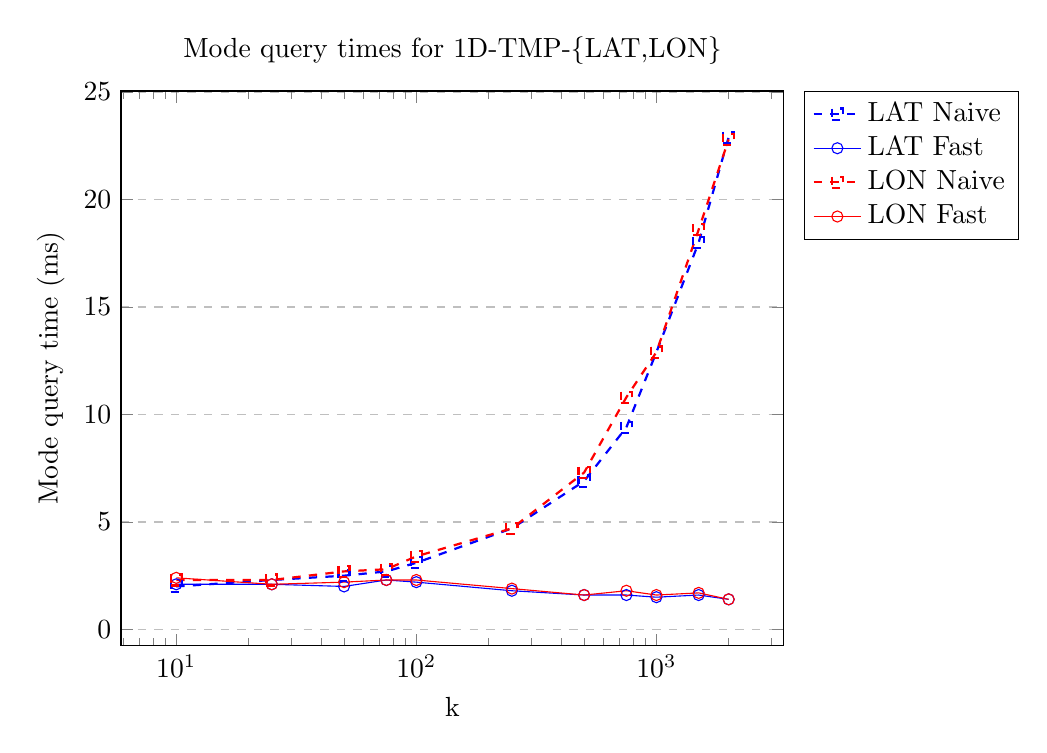
\begin{tikzpicture}
    \begin{axis}[
        title={Mode query times for 1D-TMP-\{LAT,LON\}},
        xlabel={k},xmode=log,
        ylabel={Mode query time (ms)},
        legend pos=outer north east,
        ymajorgrids=true,
        grid style=dashed,
        legend cell align={left}
    ]
    \addplot[
        color=blue,
        mark=square,
        dashed, thick,
        ]
        coordinates {
            (10, 2.0)
            (25, 2.3)
            (50, 2.5)
            (75, 2.7)
            (100, 3.1)
            (250, 4.7)
            (500, 6.9)
            (750, 9.4)
            (1000, 12.9)
            (1500, 18.0)
(2000, 22.9)
        };
    \addlegendentry{LAT Naive}
    \addplot[
        color=blue,
        mark=o,
        ]
        coordinates {
            (10, 2.1)
            (25, 2.1)
            (50, 2.0)
            (75, 2.3)
            (100, 2.2)
            (250, 1.8)
            (500, 1.6)
            (750, 1.6)
            (1000, 1.5)
            (1500, 1.6)
(2000, 1.4)
        };
    \addlegendentry{LAT Fast}
    
    \addplot[
        color=red,
        mark=square,
        dashed, thick
        ]
        coordinates {
            (10, 2.3)
            (25, 2.3)
            (50, 2.7)
            (75, 2.8)
            (100, 3.4)
            (250, 4.7)
            (500, 7.3)
            (750, 10.8)
            (1000, 12.9)
            (1500, 18.6)
(2000, 22.8)
        };
    \addlegendentry{LON Naive}
    \addplot[
        color=red,
        mark=o,
        ]
        coordinates {
            (10, 2.4)
            (25, 2.1)
            (50, 2.2)
            (75, 2.3)
            (100, 2.3)
            (250, 1.9)
            (500, 1.6)
            (750, 1.8)
            (1000, 1.6)
            (1500, 1.7)
(2000, 1.4)
        };
    \addlegendentry{LON Fast}
    \end{axis}
    \end{tikzpicture}
}

% All data

% % A1-A6
% \hskip-2cm
% \resizebox{8cm}{!}{
%     \begin{tikzpicture}
%     \begin{axis}[
%         title={Mode query times for A1-A3},
%         xlabel={k},xmode=log,
%         ylabel={Mode query time (ms)},
%         legend pos=outer north east,
%         ymajorgrids=true,
%         grid style=dashed,
%     ]
%     \addplot[
%         color=blue,
%         mark=square,
%         dashed, thick,
%         ]
%         coordinates {
%             (10, 2.2)
%             (25, 2.3)
%             (50, 2.8)
%             (75, 3.3)
%             (100, 3.3)
%             (250, 5.3)
%             (500, 7.7)
%             (750, 12.8)
%         };
%     \addlegendentry{A1 Naive}
%     \addplot[
%         color=blue,
%         mark=o,
%         ]
%         coordinates {
%             (10, 2.0)
%             (25, 1.6)
%             (50, 1.2)
%             (75, 1.3)
%             (100, 1.0)
%             (250, 0.9)
%             (500, 0.8)
%             (750, 0.8)
%         };
%     \addlegendentry{A1 Fast}
    
%     \addplot[
%         color=red,
%         mark=square,
%         dashed, thick
%         ]
%         coordinates {
%             (10, 2.3)
%             (25, 2.4)
%             (50, 2.5)
%             (75, 2.8)
%             (100, 3.0)
%             (250, 5.3)
%             (500, 7.3)
%             (750, 10.0)
%             (1000, 12.9)
%             (1500, 19.0)
%             (2000, 29.2)
%         };
%     \addlegendentry{A2 Naive}
%     \addplot[
%         color=red,
%         mark=o,
%         ]
%         coordinates {
%             (10, 2.2)
%             (25, 2.2)
%             (50, 2.3)
%             (75, 2.5)
%             (100, 2.7)
%             (250, 2.8)
%             (500, 2.3)
%             (750, 2.3)
%             (1000, 2.2)
%             (1500, 2.4)
%             (2000, 2.7)
%         };
%     \addlegendentry{A2 Fast}
    
%     \addplot[
%         color=green,
%         mark=square,
%         dashed, thick,
%         ]
%         coordinates {
%             (10, 3.9)
%             (25, 2.9)
%             (50, 3.0)
%             (75, 3.2)
%             (100, 3.7)
%             (250, 6.5)
%             (500, 11.5)
%             (750, 12.7)
%             (1000, 16.4)
%             (1500, 20.2)
% (2000, 28.7)
%         };
%     \addlegendentry{A3 Naive}
%     \addplot[
%         color=green,
%         mark=o,
%         ]
%         coordinates {
%             (10, 3.9)
%             (25, 3.0)
%             (50, 3.1)
%             (75, 3.3)
%             (100, 3.9)
%             (250, 7.8)
%             (500, 9.2)
%             (750, 8.6)
%             (1000, 8.0)
%             (1500, 7.3) 
% (2000, 8.1) 
%         };
%     \addlegendentry{A3 Fast}
%     \end{axis}
%     \end{tikzpicture}
% }
% \resizebox{8cm}{!}{
%     \begin{tikzpicture}
%     \begin{axis}[
%         title={Mode query times for A4-A6},
%         xlabel={k},xmode=log,
%         ylabel={Mode query time (ms)},
%         legend pos=outer north east,
%         ymajorgrids=true,
%         grid style=dashed,
%     ]
%     \addplot[
%         color=blue,
%         mark=square,
%         dashed, thick,
%         ]
%         coordinates {
%             (10, 2.6)
%             (25, 2.8)
%             (50, 3.1)
%             (75, 3.2)
%             (100, 3.8)
%             (250, 6.2)
%             (500, 9.9)
%             (750, 13.9)
%         };
%     \addlegendentry{A4 Naive}
%     \addplot[
%         color=blue,
%         mark=o,
%         ]
%         coordinates {
%             (10, 2.4)
%             (25, 1.9)
%             (50, 1.5)
%             (75, 1.3)
%             (100, 1.3)
%             (250, 1.1)
%             (500, 1.0)
%             (750, 0.8)
%         };
%     \addlegendentry{A4 Fast}
    
%     \addplot[
%         color=red,
%         mark=square,
%         dashed, thick
%         ]
%         coordinates {
%             (10, 2.5)
%             (25, 2.6)
%             (50, 2.9)
%             (75, 3.1)
%             (100, 3.4)
%             (250, 5.0)
%             (500, 8.3)
%             (750, 10.3)
%             (1000, 14.6)
%             (1500, 21.0)
% (2000, 29.3)
%         };
%     \addlegendentry{A5 Naive}
%     \addplot[
%         color=red,
%         mark=o,
%         ]
%         coordinates {
%             (10, 2.5)
%             (25, 2.5)
%             (50, 2.7)
%             (75, 3.2)
%             (100, 4.1)
%             (250, 3.2)
%             (500, 2.8)
%             (750, 2.6)
%             (1000, 2.5)
%             (1500, 2.9)
% (2000, 3.1)
%         };
%     \addlegendentry{A5 Fast}
    
%     \addplot[
%         color=green,
%         mark=square,
%         dashed, thick,
%         ]
%         coordinates {
%             (10, 4.0)
%             (25, 3.5)
%             (50, 3.4)
%             (75, 3.9)
%             (100, 4.2)
%             (250, 7.9)
%             (500, 10.5)
%             (750, 13.4)
%             (1000, 15.2)
%             (1500, 21.3)
% (2000, 32.3)
%         };
%     \addlegendentry{A6 Naive}
%     \addplot[
%         color=green,
%         mark=o,
%         ]
%         coordinates {
%             (10, 3.8)
%             (25, 3.7)
%             (50, 3.6)
%             (75, 4.4)
%             (100, 4.9)
%             (250, 11.0)
%             (500, 12.1)
%             (750, 11.2)
%             (1000, 9.5)
%             (1500, 9.7) 
% (2000, 10.7)
%         };
%     \addlegendentry{A6 Fast}
%     \end{axis}
%     \end{tikzpicture}
% }\\

% % A7-A12
% \hskip-2cm
% \resizebox{8cm}{!}{
%     \begin{tikzpicture}
%     \begin{axis}[
%         title={Mode query times for A7-A9},
%         xlabel={k},xmode=log,
%         ylabel={Mode query time (ms)},
%         legend pos=outer north east,
%         ymajorgrids=true,
%         grid style=dashed,
%     ]
%     \addplot[
%         color=blue,
%         mark=square,
%         dashed, thick,
%         ]
%         coordinates {
%             (10, 2.5)
%             (25, 2.9)
%             (50, 3.7)
%             (75, 3.6)
%             (100, 4.0)
%             (250, 6.4)
%             (500, 9.4)
%             (750, 14.8)
%         };
%     \addlegendentry{A7 Naive}
%     \addplot[
%         color=blue,
%         mark=o,
%         ]
%         coordinates {
%             (10, 2.1)
%             (25, 1.7)
%             (50, 1.5)
%             (75, 1.1)
%             (100, 1.0)
%             (250, 0.9)
%             (500, 0.8)
%             (750, 0.8)
%         };
%     \addlegendentry{A7 Fast}
    
%     \addplot[
%         color=red,
%         mark=square,
%         dashed, thick
%         ]
%         coordinates {
%             (10, 2.0)
%             (25, 2.2)
%             (50, 2.5)
%             (75, 3.0)
%             (100, 3.2)
%             (250, 5.1)
%             (500, 7.6)
%             (750, 10.0)
%             (1000, 12.7)
%             (1500, 21.8)
% (2000, 27.2)
%         };
%     \addlegendentry{A8 Naive}
%     \addplot[
%         color=red,
%         mark=o,
%         ]
%         coordinates {
%             (10, 1.9)
%             (25, 2.1)
%             (50, 2.2)
%             (75, 3.0)
%             (100, 3.6)
%             (250, 3.3)
%             (500, 2.3)
%             (750, 2.2)
%             (1000, 1.9)
%             (1500, 2.0) 
% (2000, 1.8) 
%         };
%     \addlegendentry{A8 Fast}
    
%     \addplot[
%         color=green,
%         mark=square,
%         dashed, thick,
%         ]
%         coordinates {
%             (10, 3.0)
%             (25, 2.7)
%             (50, 3.0)
%             (75, 4.0)
%             (100, 4.6)
%             (250, 6.1)
%             (500, 7.5)
%             (750, 10.8)
%             (1000, 14.0)
%             (1500, 22.6)
% (2000, 26.0)
%         };
%     \addlegendentry{A9 Naive}
%     \addplot[
%         color=green,
%         mark=o,
%         ]
%         coordinates {
%             (10, 3.2)
%             (25, 2.7)
%             (50, 3.0)
%             (75, 4.2)
%             (100, 4.8)
%             (250, 10.0)
%             (500, 11.1)
%             (750, 11.1)
%             (1000, 11.0)
%             (1500, 12.3)
% (2000, 9.9) 
%         };
%     \addlegendentry{A9 Fast}
%     \end{axis}
%     \end{tikzpicture}
% }
% \resizebox{8cm}{!}{
%     \begin{tikzpicture}
%     \begin{axis}[
%         title={Mode query times for A10-A12},
%         xlabel={k},xmode=log,
%         ylabel={Mode query time (ms)},
%         legend pos=outer north east,
%         ymajorgrids=true,
%         grid style=dashed,
%     ]
%     \addplot[
%         color=blue,
%         mark=square,
%         dashed, thick,
%         ]
%         coordinates {
%             (10, 3.9)
%             (25, 3.9)
%             (50, 4.6)
%             (75, 5.5)
%             (100, 5.8)
%             (250, 8.2)
%             (500, 11.0)
%             (750, 15.2)
%         };
%     \addlegendentry{A10 Naive}
%     \addplot[
%         color=blue,
%         mark=o,
%         ]
%         coordinates {
%             (10, 3.0)
%             (25, 2.3)
%             (50, 1.4)
%             (75, 1.4)
%             (100, 1.4)
%             (250, 1.1)
%             (500, 0.8)
%             (750, 0.7)
%         };
%     \addlegendentry{A10 Fast}
    
%     \addplot[
%         color=red,
%         mark=square,
%         dashed, thick
%         ]
%         coordinates {
%             (10, 2.4)
%             (25, 2.6)
%             (50, 2.8)
%             (75, 3.1)
%             (100, 3.4)
%             (250, 5.3)
%             (500, 7.7)
%             (750, 10.5)
%             (1000, 13.9)
%             (1500, 20.4)
% (2000, 27.0)
%         };
%     \addlegendentry{A11 Naive}
%     \addplot[
%         color=red,
%         mark=o,
%         ]
%         coordinates {
%            (10, 2.3)
%             (25, 2.3)
%             (50, 2.4)
%             (75, 2.7)
%             (100, 3.4)
%             (250, 2.2)
%             (500, 1.9)
%             (750, 2.0)
%             (1000, 1.8)
%             (1500, 1.9) 
% (2000, 1.7) 
%         };
%     \addlegendentry{A11 Fast}
    
%     \addplot[
%         color=green,
%         mark=square,
%         dashed, thick,
%         ]
%         coordinates {
%             (10, 3.5)
%             (25, 3.1)
%             (50, 3.3)
%             (75, 5.1)
%             (100, 4.8)
%             (250, 6.5)
%             (500, 7.9)
%             (750, 11.1)
%             (1000, 15.3)
%             (1500, 21.9)
% (2000, 26.2)
%         };
%     \addlegendentry{A12 Naive}
%     \addplot[
%         color=green,
%         mark=o,
%         ]
%         coordinates {
%             (10, 3.4)
%             (25, 3.2)
%             (50, 3.3)
%             (75, 5.1)
%             (100, 5.2)
%             (250, 9.8)
%             (500, 10.4)
%             (750, 9.8)
%             (1000, 10.1)
%             (1500, 9.2) 
% (2000, 7.6) 
%         };
%     \addlegendentry{A12 Fast}
%     \end{axis}
%     \end{tikzpicture}
% }

% % B1, B2, C1, C2
% \hskip-2cm
% \resizebox{8cm}{!}{
%     \begin{tikzpicture}
%     \begin{axis}[
%         title={Mode query times for B1 and B2},
%         xlabel={k},xmode=log,
%         ylabel={Mode query time (ms)},
%         legend pos=outer north east,
%         ymajorgrids=true,
%         grid style=dashed,
%     ]
%     \addplot[
%         color=blue,
%         mark=square,
%         dashed, thick,
%         ]
%         coordinates {
%             (1000, 14.3)
%             (2000, 26.1)
%             (3000, 37.0)
%             (4000, 48.3)
%             (5000, 59.7)
%             (6000, 75.4)
%             (7000, 80.3)
%             (8000, 98.3)
%             (9000, 112.5)
%         };
%     \addlegendentry{B1 Naive}
%     \addplot[
%         color=blue,
%         mark=o,
%         ]
%         coordinates {
%             (1000, 2.6)
%             (2000, 2.6)
%             (3000, 1.9)
%             (4000, 1.6)
%             (5000, 1.4)
%             (6000, 1.1)
%             (7000, 0.8)
%             (8000, 0.6)
%             (9000, 0.3)
%         };
%     \addlegendentry{B1 Fast}
    
%     \addplot[
%         color=red,
%         mark=square,
%         dashed, thick
%         ]
%         coordinates {
%             (1000, 14.5)
%             (2000, 28.1)
%             (3000, 39.1)
%             (4000, 48.1)
%             (5000, 59.1)
%             (6000, 74.1)
%             (7000, 82.3)
%             (8000, 96.8)
%             (9000, 110.1)
%         };
%     \addlegendentry{B2 Naive}
%     \addplot[
%         color=red,
%         mark=o,
%         ]
%         coordinates {
%             (1000, 1.8)
%             (2000, 1.7)
%             (3000, 1.4)
%             (4000, 1.1)
%             (5000, 0.9)
%             (6000, 0.8)
%             (7000, 0.6)
%             (8000, 0.4)
%             (9000, 0.2)
%         };
%     \addlegendentry{B2 Fast}
%     \end{axis}
%     \end{tikzpicture}
% }
% \resizebox{8cm}{!}{
%     \begin{tikzpicture}
%     \begin{axis}[
%         title={Mode query times for C1 and C2},
%         xlabel={k},xmode=log,
%         ylabel={Mode query time (ms)},
%         legend pos=outer north east,
%         ymajorgrids=true,
%         grid style=dashed,
%     ]
%     \addplot[
%         color=blue,
%         mark=square,
%         dashed, thick,
%         ]
%         coordinates {
%             (10, 2.0)
%             (25, 2.3)
%             (50, 2.5)
%             (75, 2.7)
%             (100, 3.1)
%             (250, 4.7)
%             (500, 6.9)
%             (750, 9.4)
%             (1000, 12.9)
%             (1500, 18.0)
% (2000, 22.9)
%         };
%     \addlegendentry{C1 Naive}
%     \addplot[
%         color=blue,
%         mark=o,
%         ]
%         coordinates {
%             (10, 2.1)
%             (25, 2.1)
%             (50, 2.0)
%             (75, 2.3)
%             (100, 2.2)
%             (250, 1.8)
%             (500, 1.6)
%             (750, 1.6)
%             (1000, 1.5)
%             (1500, 1.6)
% (2000, 1.4)
%         };
%     \addlegendentry{C1 Fast}
    
%     \addplot[
%         color=red,
%         mark=square,
%         dashed, thick
%         ]
%         coordinates {
%             (10, 2.3)
%             (25, 2.3)
%             (50, 2.7)
%             (75, 2.8)
%             (100, 3.4)
%             (250, 4.7)
%             (500, 7.3)
%             (750, 10.8)
%             (1000, 12.9)
%             (1500, 18.6)
% (2000, 22.8)
%         };
%     \addlegendentry{C2 Naive}
%     \addplot[
%         color=red,
%         mark=o,
%         ]
%         coordinates {
%             (10, 2.4)
%             (25, 2.1)
%             (50, 2.2)
%             (75, 2.3)
%             (100, 2.3)
%             (250, 1.9)
%             (500, 1.6)
%             (750, 1.8)
%             (1000, 1.6)
%             (1500, 1.7)
% (2000, 1.4)
%         };
%     \addlegendentry{C2 Fast}
%     \end{axis}
%     \end{tikzpicture}
% }


\subsubsection*{Discusssion}
For range queries, the results we see are largely expected. In Figure \ref{fig:1dresrangeartificial} we see that the naive implementation follows a roughly linear relation between $k$ and the query time, mat\fb{ch}ing our expectation of \fbrm{it being} $O(\log n + k)$. In Figure \ref{fig:1dresrangerl}a, we do see that computation time of the naive approach seems to taper off for larger $k$ values. This is most likely due to the fact that a large part of the window size for sorting is outside of array bounds as $2k > n$, thus reducing the amount of computation required. 
When looking at the range queries as described by Van der Horst et al., expectations are again met. Query time stays roughly the same over all values of $k$, and on average we see a slight increase in query time for scenarios with a larger $n$. We note that it appears that the overhead associated with the tree query is rather high, as can be seen due to the minor query time differences between $n=1000$ and $n=100,000$. In general, we see that when $k \gtrapprox 100$ the fast method seems to outperform the naive in all given figures. \\\\
\fb{
    For mode, results are also mostly in line with expectation. We do note that in Figure \ref{fig:1dresmodeartificial} we seem to see an initial jump in computation time for large $k$ with $n=1e5$, and then a decrease in computation time for even larger $k$ values. When investigating this, this bump in the curve is most likely due to there is an initial high overhead for use of the precomputed structure (when compared to doing queries that fall completely within a single precomputed span, thus using a naive counting approach). As $k$ becomes larger, this initial overhead is less pronounced causing a flattening of the curve. \\
    In general, when $k \gtrapprox 300-500$ our fast approach seems to be better than the naive.
}


\subsection{2D}
A mix of artificial and real life data was once again used in order to validate
results. As 2D datasets are generally more widely available, a larger selection
is included here as opposed to the 1D instances. \\\\ As preprocessing times
for the datastructures required for the 2D algorithms were relatively high,
graphs for these were also included. \subsubsection*{Artificial data} The same
method of generating data that was used in 1D was generalized for 2D. We refer
back to the 1D section for more details, however a couple of small changes are
highlighted.
\begin{itemize}
    \item Points were once again sampled in an arbitrarily selected range. Seeing as we
          are now in 2D, this range has been expanded to $[-50000, 50000] \times [-50000,
                  50000]$. \fbnote{As a response to Erwin's question as to why 5e4 was chosen: very much arbitrary, it was the first thing that came to mind that felt like a "nice" range + I was initially testing with integers during the 1D tree splitting fase so a range larger than [-1, 1] was required.}
    \item For the clustered color scenarios, the distance measure used for determining
          which color a point gets is $L_\infty$. This was chosen due to the fact that
          this is also the metric used in the algorithms themselves.
\end{itemize}
\fbnote{Response to feedback from Erwin: I decided to keep this section here instead of moving it due to the fact that I feel that this discussion of which $r$ is used is only interesting for these specific instances, however I do understand the critique.}
\fb{For our mode operation, we now also have an additional parameter $r$. In van der Horst et al. this value was chosen to be $\sqrt{n}$ in order to get a $O(\sqrt{n} \polylog n)$ query time, however during testing we found that preprocessing using our current implemention was exceedingly slow. We therefore decided to use a small constant $r$ instead for all artificial instances. In order to determine a suitable value, the scenario 2D-10-25-$r$-20-0-0 was selected and run with $r=\{ 5, 10, 25, 50 \}$. Larger values than this were not tested, as preprocessing times would exceed 1 hour per run of an instance. A balance between preprocessing and query time was then selected by using $r=10$, which required $~6$ seconds of preprocessing time for a single run. We refer to the raw results in the Appendix for more details on this experiment. Experiments including variable $r$ will be discussed in more detail for the real life instances.} \\\\
An overview of the tested artificial scenarios can be seen in \fb{Table \ref{tab:2dscenarios}. In this, we use a scenario naming scheme of 2D-$\{n/1000\}$-$k$-$r$-$\Delta$-$\gamma$-$\{\alpha \cdot 100\}$.}
\begin{center}
\begin{table}
    \subfloat[Uniform color scenarios]{
    \begin{tabular}{lrcccc}
        \toprule
        Scenario               & \multicolumn{1}{c}{$n$}     & $\Delta$ & $\gamma$ & $\alpha$ \\
        \cmidrule(lr){1-1} \cmidrule(lr){2-5}
        2D-1-$k$-$r$-20-0-0    & 1,000   & 20       & 0        & 0        \\
        2D-10-$k$-$r$-20-0-0   & 10,000  & 20       & 0        & 0        \\
        2D-100-$k$-$r$-20-0-0  & 100,000 & 20       & 0        & 0        \\
        2D-1-$k$-$r$-100-0-0   & 1,000   & 100      & 0        & 0        \\
        2D-10-$k$-$r$-100-0-0  & 10,000  & 100      & 0        & 0        \\
        2D-100-$k$-$r$-100-0-0 & 100,000 & 100      & 0        & 0        \\
        \bottomrule
    \end{tabular}
    }
    \:\:
    \subfloat[Clustered color scenarios]{
    \begin{tabular}{lrcccc}
        \toprule
        Scenario                  & \multicolumn{1}{c}{$n$}    & $\Delta$ & $\gamma$ & $\alpha$ \\
        \cmidrule(lr){1-1} \cmidrule(lr){2-5}
        2D-1-$k$-$r$-20-30-95     & 1,000   & 20       & 30       & 0.95     \\
        2D-10-$k$-$r$-20-30-95    & 10,000  & 20       & 30       & 0.95     \\
        2D-100-$k$-$r$-20-30-95   & 100,000 & 20       & 30       & 0.95     \\
        2D-1-$k$-$r$-100-200-95   & 1,000   & 100      & 200      & 0.95     \\
        2D-10-$k$-$r$-100-200-95  & 10,000  & 100      & 200      & 0.95     \\
        2D-100-$k$-$r$-100-200-95 & 100,000 & 100      & 200      & 0.95     \\
        \bottomrule
    \end{tabular}
    }
    \caption{\fb{Overview of 2D artificial scenarios}}
    \label{tab:2dscenarios}
\end{table}
\end{center}
\subsubsection*{Real life data}
\fb{As we already have a usable dataset in the form of the weather based one generated for 1D testing, this is reused when testing the 2D implementation. We will refer to this instance as 2D-TMP-$k$-$r$. This dataset is used in order to visualise the relation between processing and query time and as a function of $r$. For these tests, $r = \{ 2, 5, 10, 15, 20 \}$ is used.} \\\\
Additional data is however also considered, as 2D datasets are widely available. We use annotated map data as our secondary source of test data. OpenStreetMap \cite{OpenStreetMap} was used in order to download map data from 10 places in the Utrecht region, and QGIS \cite{QGIS_software} was used in order to render a simplified version of the map. See Figure \ref{fig:uithof} for an example. In selecting test data, attempts were made in order to include regions that showcased a large amount of different colors. A single test instance was also included which was mostly farmland, allowing for validation when the variation in colors is low. For more details on the exact test cases, we refer to the renderings of the selected maps which are available on GitHub \cite{vanderPlasImplementation}. \\
The map renderings were then sampled in order to produce colored points. The location of the point was taken to be the pixel coordinate in the map view image, along with a small randomized offset. This offset was uniformly sampled within a distance of 0.05 from the pixel coordinate, and was included in order to discourage exact $x$ and $y$ coordinate matches for different points. Sampling rate was set such that the total instance size was around $50,000$ points for each of the included maps. An example of the resulting sampled map can be found in Figure \ref{fig:uithof-points}. \\\\
\fb{As the amount of sample points is relatively high, we chose to generate instances based on random subsets of the full point sets. These were then used in order to visualize the dependency on $n$ seen in the algorithms by van der Horst et al. In this, $r$ was once again fixed at $10$ as was the case with the artificial test cases. We will refer to the instances as 2D-MAP-$k$-$p$, where $0 < p \leq 100$ represents the percentage of total map points used in the instance. $p=\{ 1, 5, 10, 25, 50, 75, 100 \}$ were selected in order to make instances, and each was run with the the same selection of $k$ values as used in the artificial data.} \\\\
\fb{For each instance, all maps were once again run with $Q=1000$. Results from the different maps were then averaged in order to produce computation times for a certain instance.}


\begin{figure}[!tbp]
    \centering
    \subfloat[Simplified map view of Utrecht Science Park, centered on the Buys Ballot Building.]{\includegraphics[width=0.45\textwidth]{figs/usp.png}\label{fig:uithof}}
    \hfill
    \subfloat[Point sampling taking from the simplified map view.]{\includegraphics[width=0.45\textwidth]{figs/usp_points.png}\label{fig:uithof-points}}
    \caption{2D map data to pointset conversion}
\end{figure}

\subsubsection*{Results}

% A1-6
\begin{figure}[H]
    \begin{center}
        \subfloat[2D-\{1,10,100\}-$k$-10-20-0-0]{
            \resizebox{8cm}{!}{
                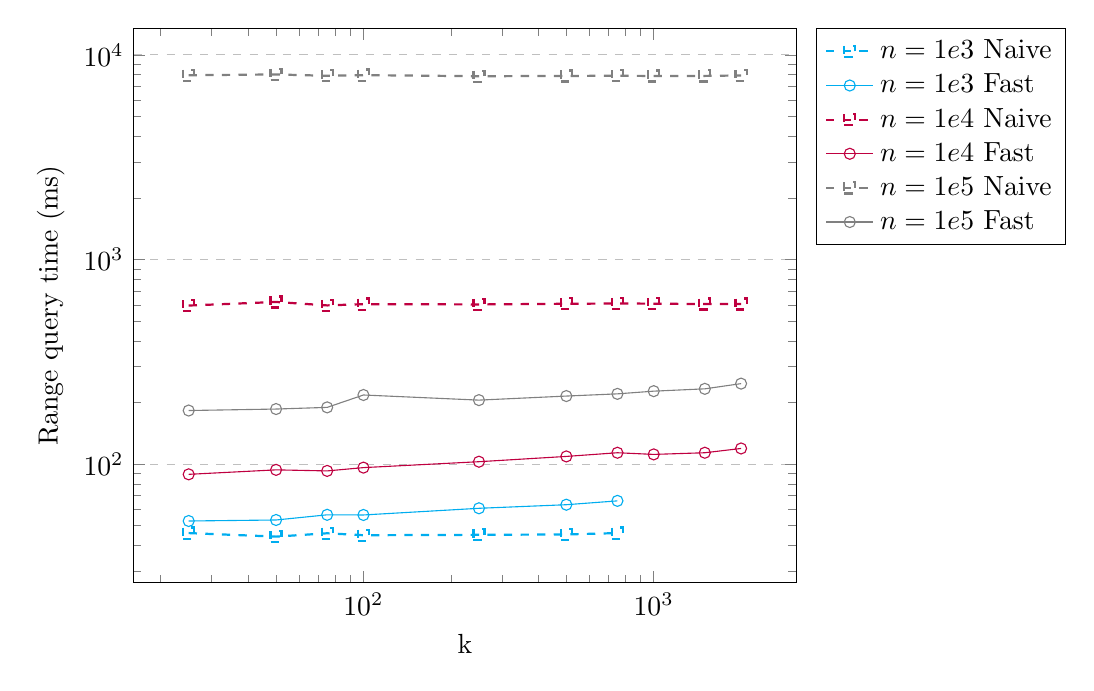
\begin{tikzpicture}
                    \begin{axis}[
                            xmode=log,
                            ymode=log,
                            xlabel={k},
                            ylabel={Range query time (ms)},
                            legend pos=outer north east,
                            ymajorgrids=true,
                            grid style=dashed,
                            legend cell align={left},
                        ]
                        \addplot[
                            color=cyan,
                            mark=square,
                            dashed, thick,
                        ]
                        coordinates {
                                (25, 46.0)
                                (50, 44.2)
                                (75, 45.9)
                                (100, 44.9)
                                (250, 45.1)
                                (500, 45.3)
                                (750, 46.0)
                            };
                        \addlegendentry{$n=1e3$ Naive}
                        \addplot[
                            color=cyan,
                            mark=o,
                        ]
                        coordinates {
                                (25, 52.7)
                                (50, 53.3)
                                (75, 56.5)
                                (100, 56.4)
                                (250, 60.8)
                                (500, 63.3)
                                (750, 66.1)
                            };
                        \addlegendentry{$n=1e3$ Fast}

                        \addplot[
                            color=purple,
                            mark=square,
                            dashed, thick
                        ]
                        coordinates {
                                (25, 595.5)
                                (50, 620.0)
                                (75, 596.4)
                                (100, 605.0)
                                (250, 603.0)
                                (500, 607.4)
                                (750, 609.4)
                                (1000, 608.1)
                                (1500, 605.5)
                                (2000, 605.5)
                            };
                        \addlegendentry{$n=1e4$ Naive}
                        \addplot[
                            color=purple,
                            mark=o,
                        ]
                        coordinates {
                                (25, 89.1)
                                (50, 93.7)
                                (75, 92.6)
                                (100, 96.1)
                                (250, 102.7)
                                (500, 109.0)
                                (750, 113.6)
                                (1000, 111.5)
                                (1500, 113.6)
                                (2000, 119.2)
                            };
                        \addlegendentry{$n=1e4$ Fast}

                        \addplot[
                            color=gray,
                            mark=square,
                            dashed, thick,
                        ]
                        coordinates {
                                (25, 7952.8)
                                (50, 8024.1)
                                (75, 7903.2)
                                (100, 7961.9)
                                (250, 7866.1)
                                (500, 7888.8)
                                (750, 7909.8)
                                (1000, 7887.2)
                                (1500, 7894.8)
                                (2000, 7935.7)
                            };
                        \addlegendentry{$n=1e5$ Naive}
                        \addplot[
                            color=gray,
                            mark=o,
                        ]
                        coordinates {
                                (25, 182.7)
                                (50, 185.8)
                                (75, 189.3)
                                (100, 217.6)
                                (250, 205.4)
                                (500, 215.0)
                                (750, 220.4)
                                (1000, 227.2)
                                (1500, 233.2)
                                (2000, 247.3)
                            };
                        \addlegendentry{$n=1e5$ Fast}
                    \end{axis}
                \end{tikzpicture}
            }}
        \subfloat[2D-\{1,10,100\}-$k$-10-100-200-95]{
            \resizebox{8cm}{!}{
                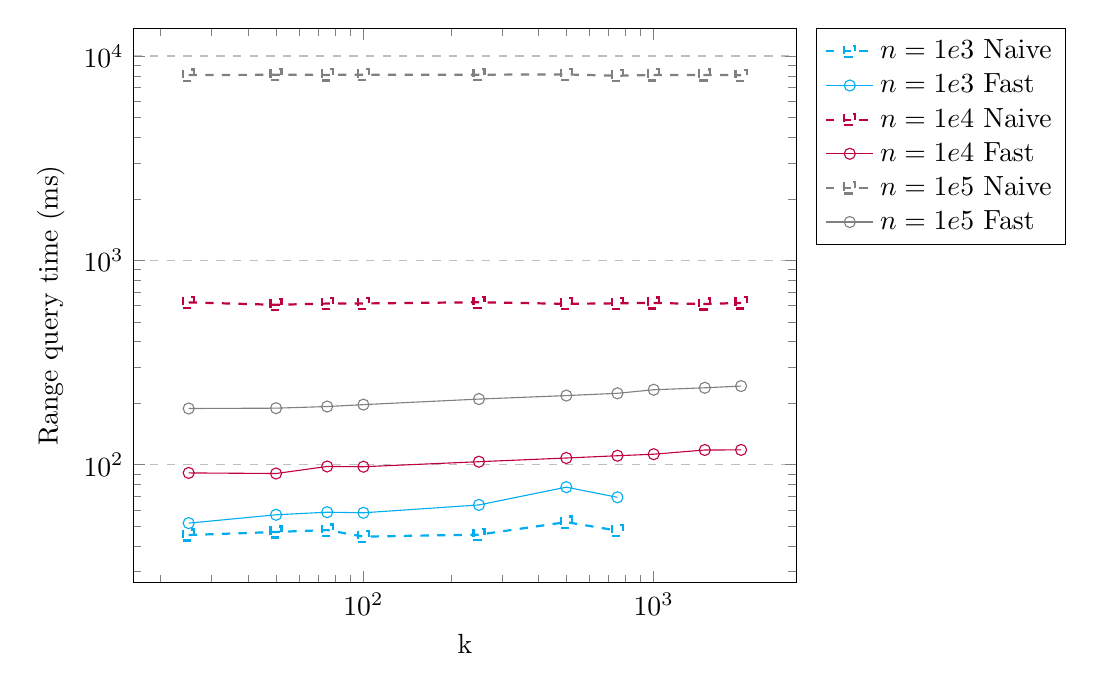
\begin{tikzpicture}
                    \begin{axis}[
                            xmode=log,
                            ymode=log,
                            xlabel={k},
                            ylabel={Range query time (ms)},
                            legend pos=outer north east,
                            ymajorgrids=true,
                            grid style=dashed,
                            legend cell align={left},
                        ]
                        \addplot[
                            color=cyan,
                            mark=square,
                            dashed, thick,
                        ]
                        coordinates {
                                (25, 45.3)
                                (50, 46.9)
                                (75, 47.9)
                                (100, 44.5)
                                (250, 45.5)
                                (500, 52.4)
                                (750, 47.6)
                            };
                        \addlegendentry{$n=1e3$ Naive}
                        \addplot[
                            color=cyan,
                            mark=o,
                        ]
                        coordinates {
                                (25, 51.8)
                                (50, 56.9)
                                (75, 58.6)
                                (100, 58.2)
                                (250, 63.6)
                                (500, 77.7)
                                (750, 69.3)
                            };
                        \addlegendentry{$n=1e3$ Fast}

                        \addplot[
                            color=purple,
                            mark=square,
                            dashed, thick
                        ]
                        coordinates {
                                (25, 623.1)
                                (50, 606.2)
                                (75, 614.9)
                                (100, 615.4)
                                (250, 624.2)
                                (500, 612.8)
                                (750, 616.6)
                                (1000, 619.2)
                                (1500, 611.5)
                                (2000, 619.7)
                            };
                        \addlegendentry{$n=1e4$ Naive}
                        \addplot[
                            color=purple,
                            mark=o,
                        ]
                        coordinates {
                                (25, 91.2)
                                (50, 90.6)
                                (75, 98.1)
                                (100, 97.8)
                                (250, 103.5)
                                (500, 107.9)
                                (750, 110.7)
                                (1000, 112.6)
                                (1500, 118.1)
                                (2000, 118.2)
                            };
                        \addlegendentry{$n=1e4$ Fast}

                        \addplot[
                            color=gray,
                            mark=square,
                            dashed, thick,
                        ]
                        coordinates {
                                (25, 8066.8)
                                (50, 8097.7)
                                (75, 8084.5)
                                (100, 8098.0)
                                (250, 8103.3)
                                (500, 8126.7)
                                (750, 8006.5)
                                (1000, 8082.0)
                                (1500, 8074.1)
                                (2000, 8060.0)
                            };
                        \addlegendentry{$n=1e5$ Naive}
                        \addplot[
                            color=gray,
                            mark=o,
                        ]
                        coordinates {
                                (25, 188.5)
                                (50, 189.2)
                                (75, 192.7)
                                (100, 196.9)
                                (250, 209.6)
                                (500, 218.0)
                                (750, 223.7)
                                (1000, 232.8)
                                (1500, 238.0)
                                (2000, 242.7)
                            };
                        \addlegendentry{$n=1e5$ Fast}
                    \end{axis}
                \end{tikzpicture}
            }}
    \end{center}
    \caption{Naive and fast mode query times on 2D artificial instances}
    \label{fig:2dresrangeartificial}
\end{figure}

\begin{figure}[H]
    \begin{center}
        \subfloat[2D-MAP-$k$-$p$, multiple $k$ values displayed for a single $n$]{
            \resizebox{8cm}{!}{
                \begin{tikzpicture}
                    \begin{axis}[
                            xmode=log,
                            ymode=log,
                            xlabel={n},
                            ylabel={Range query time (ms)},
                            legend pos=outer north east,
                            ymajorgrids=true,
                            grid style=dashed,
                            legend cell align={left},
                        ]
                        \addplot[
                            color=cyan,
                            mark=square,
                            dashed, thick,
                            only marks
                        ]
                        coordinates {
                            (500, 21.0)
(500, 21.9)
(500, 20.7)
(500, 21.0)
(500, 21.5)

(2500, 143.6)
(2500, 145.9)
(2500, 153.4)
(2500, 153.6)
(2500, 146.1)
(2500, 162.1)
(2500, 148.8)
(2500, 158.3)
(2500, 153.5)
(2500, 158.3)

(5000, 329.1)
(5000, 339.4)
(5000, 321.8)
(5000, 323.9)
(5000, 325.9)
(5000, 321.3)
(5000, 327.7)
(5000, 329.9)
(5000, 333.8)
(5000, 323.4)

(12500, 881.6)
(12500, 871.4)
(12500, 846.7)
(12500, 848.9)
(12500, 846.6)
(12500, 893.6)
(12500, 893.1)
(12500, 891.4)
(12500, 890.3)
(12500, 929.9)

(25000, 2054.7)
(25000, 2115.4)
(25000, 1918.2)
(25000, 1924.5)
(25000, 2100.5)
(25000, 1923.4)
(25000, 1805.0)
(25000, 1889.8)
(25000, 2108.4)
(25000, 1977.8)

(37500, 3198.7)
(37500, 2958.2)
(37500, 2970.9)
(37500, 3069.6)
(37500, 3068.3)
(37500, 3107.8)
(37500, 3088.4)
(37500, 3040.5)
(37500, 2834.7)
(37500, 3059.2)

(50000, 4328.7)
(50000, 4503.1)
(50000, 4152.4)
(50000, 4128.6)
(50000, 4069.3)
(50000, 4273.2)
(50000, 4183.3)
(50000, 4105.4)
(50000, 3998.4)
(50000, 3856.8)
                            };
                        \addlegendentry{Naive}
                        \addplot[
                            color=purple,
                            mark=o,
                            only marks,
                        ]
                        coordinates {
                            (500, 45.5)
                            (500, 52.1)
                            (500, 50.0)
                            (500, 50.4)
                            (500, 54.8)
                            (2500, 67.0)
                            (2500, 68.0)
                            (2500, 81.1)
                            (2500, 80.0)
                            (2500, 80.1)
                            (2500, 94.4)
                            (2500, 90.4)
                            (2500, 92.2)
                            (2500, 92.0)
                            (2500, 99.3)
                            (5000, 82.0)
                            (5000, 87.4)
                            (5000, 87.5)
                            (5000, 88.8)
                            (5000, 96.8)
                            (5000, 98.9)
                            (5000, 104.5)
                            (5000, 109.0)
                            (5000, 113.6)
                            (5000, 108.7)
                            (12500, 98.3)
                            (12500, 101.0)
                            (12500, 98.2)
                            (12500, 100.3)
                            (12500, 108.5)
                            (12500, 119.5)
                            (12500, 128.1)
                            (12500, 126.6)
                            (12500, 132.4)
                            (12500, 141.5)
                            (25000, 120.2)
                            (25000, 136.6)
                            (25000, 131.0)
                            (25000, 134.2)
                            (25000, 152.2)
                            (25000, 142.7)
                            (25000, 140.3)
                            (25000, 147.0)
                            (25000, 178.7)
                            (25000, 166.4)
                            (37500, 154.4)
                            (37500, 137.0)
                            (37500, 141.7)
                            (37500, 152.5)
                            (37500, 155.3)
                            (37500, 164.8)
                            (37500, 171.8)
                            (37500, 166.4)
                            (37500, 160.4)
                            (37500, 167.5)
                            (50000, 151.0)
                            (50000, 160.3)
                            (50000, 155.9)
                            (50000, 162.7)
                            (50000, 172.3)
                            (50000, 181.8)
                            (50000, 175.0)
                            (50000, 183.2)
                            (50000, 177.2)
                            (50000, 174.6)
                            };
                        \addlegendentry{Fast}
                    \end{axis}
                \end{tikzpicture}
            }}
    \end{center}
    \caption{Naive and fast range query times on 2D real life map instances. Plotted against $n$. Temperature instances not considered as range has no dependency on $r$.}
    \label{fig:2dresrangerl}
\end{figure}
% All data
% % A1-6
% \hskip-2cm
% \resizebox{8cm}{!}{
%     \begin{tikzpicture}
%     \begin{axis}[
%         title={Range query times for 1-3},
%         xmode=log,
%         ymode=log,
%         xlabel={k},
%         ylabel={Range query time (ms)},
%         legend pos=outer north east,
%         ymajorgrids=true,
%         grid style=dashed,
%     ]
%     \addplot[
%         color=cyan,
%         mark=square,
%         dashed, thick,
%         ]
%         coordinates {
%             (25, 5.2)
% (50, 14.0)
% (75, 20.1)
% (100, 26.2)
% (250, 68.6)
% (500, 137.1)
% (750, 211.0)
%         };
%     \addlegendentry{1 Naive}
%     \addplot[
%         color=cyan,
%         mark=o,
%         ]
%         coordinates {
%             (25, 55.0)
% (50, 54.1)
% (75, 57.8)
% (100, 59.7)
% (250, 64.0)
% (500, 67.2)
% (750, 65.8)
%         };
%     \addlegendentry{1 Fast}

%     \addplot[
%         color=purple,
%         mark=square,
%         dashed, thick
%         ]
%         coordinates {
%             (25, 5.2)
% (50, 10.5)
% (75, 16.6)
% (100, 22.1)
% (250, 60.4)
% (500, 126.4)
% (750, 204.6)
% (1000, 275.9)
% (1500, 436.0)
% (2000, 616.6)
%         };
%     \addlegendentry{2 Naive}
%     \addplot[
%         color=purple,
%         mark=o,
%         ]
%         coordinates {
%             (25, 105.2)
% (50, 97.7)
% (75, 99.3)
% (100, 100.1)
% (250, 103.8)
% (500, 109.6)
% (750, 123.8)
% (1000, 113.4)
% (1500, 122.7)
% (2000, 132.5)
%         };
%     \addlegendentry{2 Fast}

%     \addplot[
%         color=gray,
%         mark=square,
%         dashed, thick,
%         ]
%         coordinates {
%             (25, 5.5)
% (50, 10.6)
% (75, 17.6)
% (100, 25.3)
% (250, 63.0)
% (500, 133.9)
% (750, 206.6)
% (1000, 279.0)
% (1500, 429.1)
% (2000, 593.1)
%         };
%     \addlegendentry{3 Naive}
%     \addplot[
%         color=gray,
%         mark=o,
%         ]
%         coordinates {
%           (25, 211.0)
% (50, 194.2)
% (75, 211.8)
% (100, 230.2)
% (250, 218.6)
% (500, 225.7)
% (750, 223.5)
% (1000, 227.0)
% (1500, 236.0)
% (2000, 237.0)  
%         };
%     \addlegendentry{3 Fast}
%     \end{axis}
%     \end{tikzpicture}
% }
% \resizebox{8cm}{!}{
%     \begin{tikzpicture}
%     \begin{axis}[
%         title={Range query times for 4-6},
%         xmode=log,
%         ymode=log,
%         xlabel={k},
%         ylabel={Range query time (ms)},
%         legend pos=outer north east,
%         ymajorgrids=true,
%         grid style=dashed,
%     ]
%     \addplot[
%         color=cyan,
%         mark=square,
%         dashed, thick,
%         ]
%         coordinates {
%             (25, 5.1)
% (50, 11.7)
% (75, 17.6)
% (100, 23.6)
% (250, 62.7)
% (500, 125.8)
% (750, 200.5)
%         };
%     \addlegendentry{4 Naive}
%     \addplot[
%         color=cyan,
%         mark=o,
%         ]
%         coordinates {
%             (25, 50.4)
% (50, 52.5)
% (75, 53.4)
% (100, 54.9)
% (250, 60.1)
% (500, 61.0)
% (750, 63.1)
%         };
%     \addlegendentry{4 Fast}

%     \addplot[
%         color=purple,
%         mark=square,
%         dashed, thick
%         ]
%         coordinates {
%             (25, 5.1)
% (50, 10.4)
% (75, 15.8)
% (100, 21.9)
% (250, 59.1)
% (500, 124.3)
% (750, 201.0)
% (1000, 275.1)
% (1500, 429.8)
% (2000, 585.2)
%         };
%     \addlegendentry{5 Naive}
%     \addplot[
%         color=purple,
%         mark=o,
%         ]
%         coordinates {
%             (25, 85.8)
% (50, 89.0)
% (75, 90.0)
% (100, 93.3)
% (250, 100.0)
% (500, 104.9)
% (750, 105.7)
% (1000, 109.6)
% (1500, 111.5)
% (2000, 114.3)
%         };
%     \addlegendentry{5 Fast}

%     \addplot[
%         color=gray,
%         mark=square,
%         dashed, thick,
%         ]
%         coordinates {
%             (25, 5.3)
% (50, 11.7)
% (75, 16.5)
% (100, 22.6)
% (250, 60.6)
% (500, 129.8)
% (750, 203.2)
% (1000, 276.0)
% (1500, 441.6)
% (2000, 592.7)
%         };
%     \addlegendentry{6 Naive}
%     \addplot[
%         color=gray,
%         mark=o,
%         ]
%         coordinates {
%             (25, 176.2)
% (50, 187.3)
% (75, 189.0)
% (100, 194.3)
% (250, 204.3)
% (500, 217.3)
% (750, 225.0)
% (1000, 227.5)
% (1500, 249.7)
% (2000, 237.2)
%         };
%     \addlegendentry{6 Fast}
%     \end{axis}
%     \end{tikzpicture}
% }

% % 7-12
% \hskip-2cm
% \resizebox{8cm}{!}{
%     \begin{tikzpicture}
%     \begin{axis}[
%         title={Range query times for 7-9},
%         xmode=log,
%         ymode=log,
%         xlabel={k},
%         ylabel={Range query time (ms)},
%         legend pos=outer north east,
%         ymajorgrids=true,
%         grid style=dashed,
%     ]
%     \addplot[
%         color=cyan,
%         mark=square,
%         dashed, thick,
%         ]
%         coordinates {
%             (25, 4.9)
% (50, 12.2)
% (75, 17.7)
% (100, 23.7)
% (250, 62.2)
% (500, 129.2)
% (750, 200.8)
%         };
%     \addlegendentry{7 Naive}
%     \addplot[
%         color=cyan,
%         mark=o,
%         ]
%         coordinates {
%             (25, 49.2)
% (50, 53.6)
% (75, 54.4)
% (100, 54.6)
% (250, 59.2)
% (500, 62.2)
% (750, 63.0)
%         };
%     \addlegendentry{7 Fast}

%     \addplot[
%         color=purple,
%         mark=square,
%         dashed, thick
%         ]
%         coordinates {
%             (25, 5.0)
% (50, 10.3)
% (75, 16.2)
% (100, 22.0)
% (250, 58.5)
% (500, 123.5)
% (750, 197.7)
% (1000, 266.9)
% (1500, 421.8)
% (2000, 585.5)
%         };
%     \addlegendentry{8 Naive}
%     \addplot[
%         color=purple,
%         mark=o,
%         ]
%         coordinates {
%             (25, 85.8)
% (50, 90.2)
% (75, 91.3)
% (100, 96.7)
% (250, 99.1)
% (500, 105.6)
% (750, 105.4)
% (1000, 110.0)
% (1500, 110.2)
% (2000, 116.9)
%         };
%     \addlegendentry{8 Fast}

%     \addplot[
%         color=gray,
%         mark=square,
%         dashed, thick,
%         ]
%         coordinates {
%             (25, 5.4)
% (50, 10.9)
% (75, 16.2)
% (100, 23.2)
% (250, 60.8)
% (500, 130.3)
% (750, 200.0)
% (1000, 275.7)
% (1500, 441.0)
% (2000, 600.9)
%         };
%     \addlegendentry{9 Naive}
%     \addplot[
%         color=gray,
%         mark=o,
%         ]
%         coordinates {
%             (25, 178.7)
% (50, 188.4)
% (75, 190.0)
% (100, 196.2)
% (250, 207.9)
% (500, 219.9)
% (750, 225.7)
% (1000, 226.9)
% (1500, 232.9)
% (2000, 239.3)
%         };
%     \addlegendentry{9 Fast}
%     \end{axis}
%     \end{tikzpicture}
% }
% \resizebox{8cm}{!}{
%     \begin{tikzpicture}
%     \begin{axis}[
%         title={Range query times for 10-12},
%         xmode=log,
%         ymode=log,
%         xlabel={k},
%         ylabel={Range query time (ms)},
%         legend pos=outer north east,
%         ymajorgrids=true,
%         grid style=dashed,
%     ]
%     \addplot[
%         color=cyan,
%         mark=square,
%         dashed, thick,
%         ]
%         coordinates {
%             (25, 5.0)
% (50, 12.0)
% (75, 17.9)
% (100, 24.0)
% (250, 62.8)
% (500, 131.3)
% (750, 202.3)
%         };
%     \addlegendentry{10 Naive}
%     \addplot[
%         color=cyan,
%         mark=o,
%         ]
%         coordinates {
%             (25, 50.2)
% (50, 53.2)
% (75, 55.6)
% (100, 57.2)
% (250, 60.4)
% (500, 63.9)
% (750, 63.2)
%         };
%     \addlegendentry{10 Fast}

%     \addplot[
%         color=purple,
%         mark=square,
%         dashed, thick
%         ]
%         coordinates {
%             (25, 5.0)
% (50, 10.6)
% (75, 16.6)
% (100, 22.1)
% (250, 58.7)
% (500, 123.4)
% (750, 201.9)
% (1000, 275.5)
% (1500, 432.5)
% (2000, 587.5)
%         };
%     \addlegendentry{11 Naive}
%     \addplot[
%         color=purple,
%         mark=o,
%         ]
%         coordinates {
%             (25, 84.5)
% (50, 92.5)
% (75, 93.8)
% (100, 92.7)
% (250, 101.9)
% (500, 108.0)
% (750, 109.9)
% (1000, 109.9)
% (1500, 115.2)
% (2000, 112.8)
%         };
%     \addlegendentry{11 Fast}

%     \addplot[
%         color=gray,
%         mark=square,
%         dashed, thick,
%         ]
%         coordinates {
%             (25, 5.2)
% (50, 11.0)
% (75, 16.4)
% (100, 22.4)
% (250, 60.5)
% (500, 125.4)
% (750, 198.1)
% (1000, 279.6)
% (1500, 432.0)
% (2000, 586.9)
%         };
%     \addlegendentry{12 Naive}
%     \addplot[
%         color=gray,
%         mark=o,
%         ]
%         coordinates {
%             (25, 177.2)
% (50, 187.2)
% (75, 190.4)
% (100, 196.8)
% (250, 209.2)
% (500, 217.1)
% (750, 227.6)
% (1000, 229.2)
% (1500, 239.1)
% (2000, 239.0)
%         };
%     \addlegendentry{12 Fast}
%     \end{axis}
%     \end{tikzpicture}
% }

% A1-6
\hskip-2cm
\resizebox{8cm}{!}{
    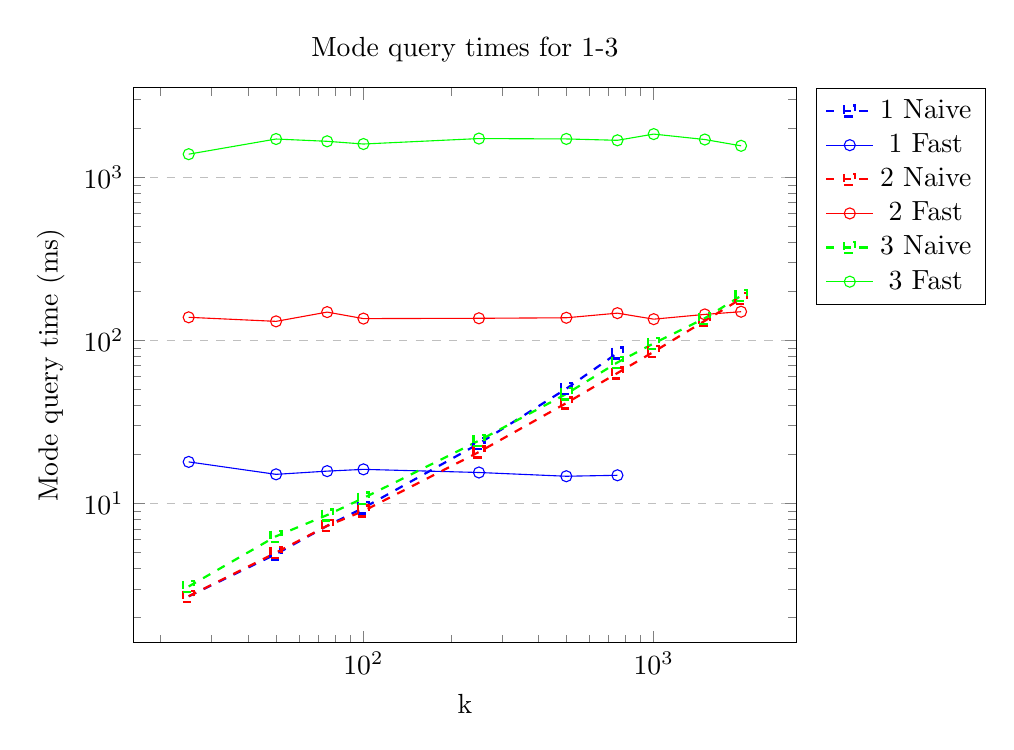
\begin{tikzpicture}
    \begin{axis}[
        title={Mode query times for 1-3},
        xmode=log,
        ymode=log,
        xlabel={k},
        ylabel={Mode query time (ms)},
        legend pos=outer north east,
        ymajorgrids=true,
        grid style=dashed,
    ]
    \addplot[
        color=blue,
        mark=square,
        dashed, thick,
        ]
        coordinates {
            (25, 2.7)
(50, 4.9)
(75, 7.3)
(100, 9.4)
(250, 23.3)
(500, 50.6)
(750, 83.7)
        };
    \addlegendentry{1 Naive}
    \addplot[
        color=blue,
        mark=o,
        ]
        coordinates {
            (25, 18.0)
(50, 15.1)
(75, 15.8)
(100, 16.2)
(250, 15.5)
(500, 14.7)
(750, 14.9)
        };
    \addlegendentry{1 Fast}
    
    \addplot[
        color=red,
        mark=square,
        dashed, thick
        ]
        coordinates {
            (25, 2.7)
(50, 5.0)
(75, 7.3)
(100, 9.0)
(250, 20.7)
(500, 41.3)
(750, 63.1)
(1000, 85.2)
(1500, 131.9)
(2000, 180.0)
        };
    \addlegendentry{2 Naive}
    \addplot[
        color=red,
        mark=o,
        ]
        coordinates {
        (25, 138.6)
(50, 130.9)
(75, 149.2)
(100, 136.1)
(250, 136.7)
(500, 137.7)
(750, 147.0)
(1000, 135.0)
(1500, 144.4)
(2000, 150.0)
        };
    \addlegendentry{2 Fast}
    
    \addplot[
        color=green,
        mark=square,
        dashed, thick,
        ]
        coordinates {
            (25, 3.1)
(50, 6.3)
(75, 8.5)
(100, 10.8)
(250, 24.3)
(500, 47.0)
(750, 73.3)
(1000, 95.9)
(1500, 136.8)
(2000, 187.7)
        };
    \addlegendentry{3 Naive}
    \addplot[
        color=green,
        mark=o,
        ]
        coordinates {
            (25, 1386.5)
(50, 1717.8)
(75, 1663.1)
(100, 1600.7)
(250, 1728.6)
(500, 1719.6)
(750, 1686.8)
(1000, 1841.6)
(1500, 1705.7)
(2000, 1560.6)
        };
    \addlegendentry{3 Fast}
    \end{axis}
    \end{tikzpicture}
}
\resizebox{8cm}{!}{
    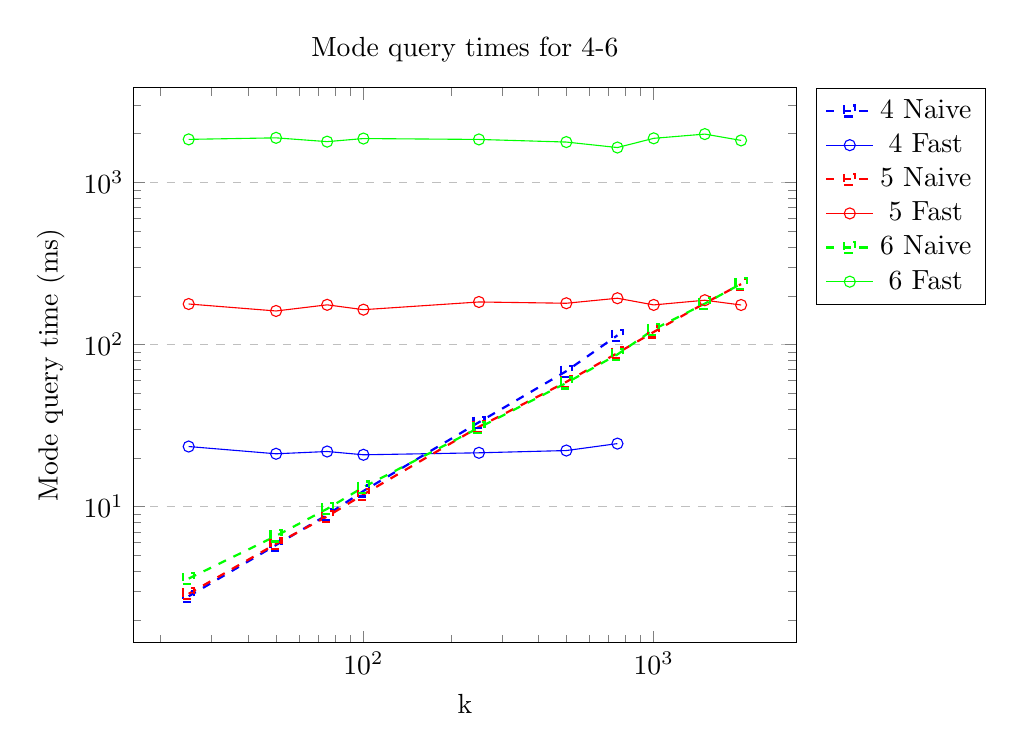
\begin{tikzpicture}
    \begin{axis}[
        title={Mode query times for 4-6},
        xmode=log,
        ymode=log,
        xlabel={k},
        ylabel={Mode query time (ms)},
        legend pos=outer north east,
        ymajorgrids=true,
        grid style=dashed,
    ]
    \addplot[
        color=blue,
        mark=square,
        dashed, thick,
        ]
        coordinates {
            (25, 2.8)
(50, 5.8)
(75, 8.9)
(100, 12.5)
(250, 33.2)
(500, 68.6)
(750, 114.1)
        };
    \addlegendentry{4 Naive}
    \addplot[
        color=blue,
        mark=o,
        ]
        coordinates {
            (25, 23.5)
(50, 21.2)
(75, 21.9)
(100, 20.9)
(250, 21.5)
(500, 22.2)
(750, 24.5)
        };
    \addlegendentry{4 Fast}
    
    \addplot[
        color=red,
        mark=square,
        dashed, thick
        ]
        coordinates {
            (25, 2.9)
(50, 5.9)
(75, 8.7)
(100, 11.9)
(250, 31.1)
(500, 58.9)
(750, 88.7)
(1000, 119.7)
(1500, 180.3)
(2000, 236.2)
        };
    \addlegendentry{5 Naive}
    \addplot[
        color=red,
        mark=o,
        ]
        coordinates {
            (25, 178.1)
(50, 161.3)
(75, 176.0)
(100, 164.3)
(250, 183.3)
(500, 180.0)
(750, 193.3)
(1000, 175.8)
(1500, 187.9)
(2000, 175.6)
        };
    \addlegendentry{5 Fast}
    
    \addplot[
        color=green,
        mark=square,
        dashed, thick,
        ]
        coordinates {
            (25, 3.6)
(50, 6.6)
(75, 9.7)
(100, 13.2)
(250, 30.7)
(500, 58.0)
(750, 87.0)
(1000, 124.1)
(1500, 179.0)
(2000, 237.4)
        };
    \addlegendentry{6 Naive}
    \addplot[
        color=green,
        mark=o,
        ]
        coordinates {
            (25, 1847.2)
(50, 1887.8)
(75, 1788.6)
(100, 1868.8)
(250, 1845.6)
(500, 1778.1)
(750, 1644.8)
(1000, 1875.0)
(1500, 1991.3)
(2000, 1820.0)
        };
    \addlegendentry{6 Fast}
    \end{axis}
    \end{tikzpicture}
}

% 7-12
\hskip-2cm
\resizebox{8cm}{!}{
    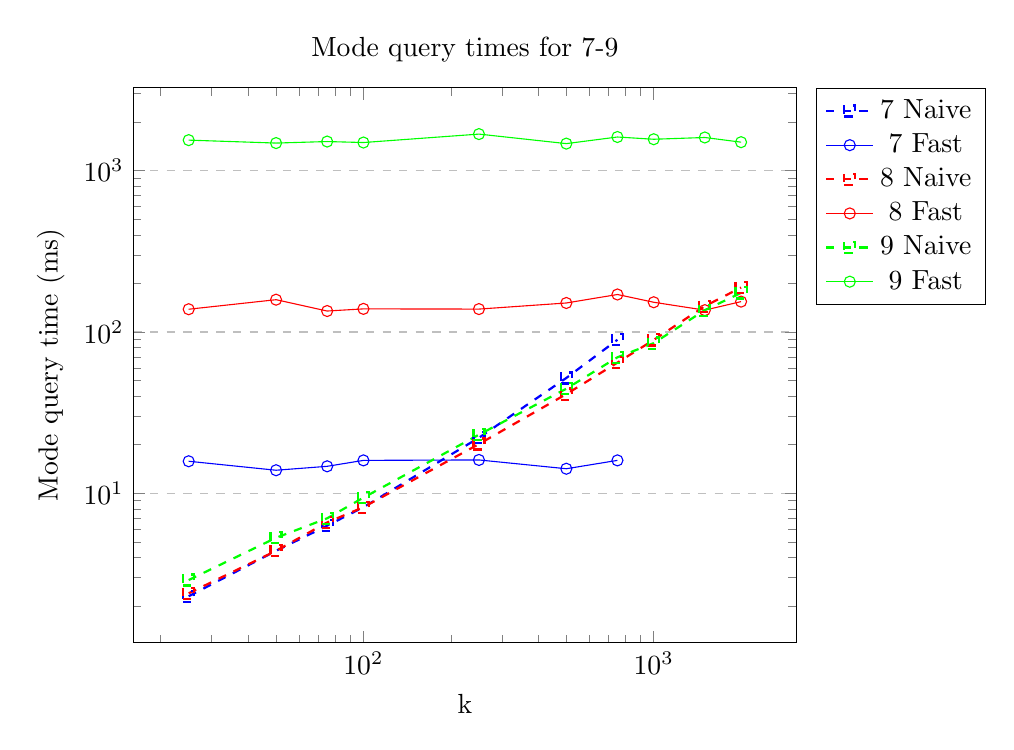
\begin{tikzpicture}
    \begin{axis}[
        title={Mode query times for 7-9},
        xmode=log,
        ymode=log,
        xlabel={k},
        ylabel={Mode query time (ms)},
        legend pos=outer north east,
        ymajorgrids=true,
        grid style=dashed,
    ]
    \addplot[
        color=blue,
        mark=square,
        dashed, thick,
        ]
        coordinates {
            (25, 2.3)
(50, 4.4)
(75, 6.3)
(100, 8.2)
(250, 22.1)
(500, 51.9)
(750, 89.5)
        };
    \addlegendentry{7 Naive}
    \addplot[
        color=blue,
        mark=o,
        ]
        coordinates {
            (25, 15.8)
(50, 13.9)
(75, 14.7)
(100, 16.0)
(250, 16.1)
(500, 14.2)
(750, 16.0)
        };
    \addlegendentry{7 Fast}
    
    \addplot[
        color=red,
        mark=square,
        dashed, thick
        ]
        coordinates {
            (25, 2.4)
(50, 4.4)
(75, 6.6)
(100, 8.2)
(250, 20.2)
(500, 41.2)
(750, 64.6)
(1000, 89.3)
(1500, 144.5)
(2000, 188.7)
        };
    \addlegendentry{8 Naive}
    \addplot[
        color=red,
        mark=o,
        ]
        coordinates {
            (25, 138.4)
(50, 158.6)
(75, 134.9)
(100, 139.1)
(250, 138.7)
(500, 151.3)
(750, 170.8)
(1000, 152.9)
(1500, 136.6)
(2000, 154.3)
        };
    \addlegendentry{8 Fast}
    
    \addplot[
        color=green,
        mark=square,
        dashed, thick,
        ]
        coordinates {
            (25, 2.9)
(50, 5.3)
(75, 7.0)
(100, 9.4)
(250, 23.1)
(500, 44.5)
(750, 69.7)
(1000, 85.3)
(1500, 136.6)
(2000, 174.8)
        };
    \addlegendentry{9 Naive}
    \addplot[
        color=green,
        mark=o,
        ]
        coordinates {
            (25, 1546.9)
(50, 1483.5)
(75, 1516.0)
(100, 1494.9)
(250, 1686.3)
(500, 1471.9)
(750, 1617.5)
(1000, 1566.5)
(1500, 1606.4)
(2000, 1502.5)
        };
    \addlegendentry{9 Fast}
    \end{axis}
    \end{tikzpicture}
}
\resizebox{8cm}{!}{
    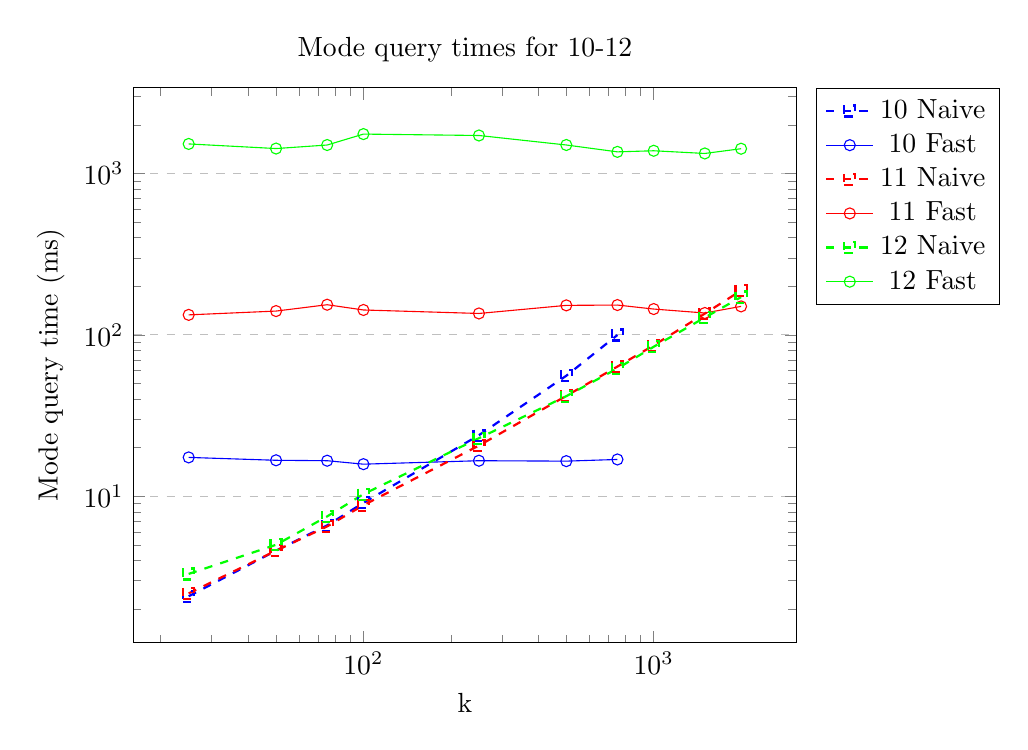
\begin{tikzpicture}
    \begin{axis}[
        title={Mode query times for 10-12},
        xmode=log,
        ymode=log,
        xlabel={k},
        ylabel={Mode query time (ms)},
        legend pos=outer north east,
        ymajorgrids=true,
        grid style=dashed,
    ]
    \addplot[
        color=blue,
        mark=square,
        dashed, thick,
        ]
        coordinates {
            (25, 2.4)
(50, 4.6)
(75, 6.6)
(100, 9.1)
(250, 23.9)
(500, 55.8)
(750, 99.8)
        };
    \addlegendentry{10 Naive}
    \addplot[
        color=blue,
        mark=o,
        ]
        coordinates {
            (25, 17.4)
(50, 16.7)
(75, 16.6)
(100, 15.8)
(250, 16.6)
(500, 16.5)
(750, 16.9)
        };
    \addlegendentry{10 Fast}
    
    \addplot[
        color=red,
        mark=square,
        dashed, thick
        ]
        coordinates {
            (25, 2.5)
(50, 4.6)
(75, 6.5)
(100, 8.8)
(250, 20.6)
(500, 41.9)
(750, 63.6)
(1000, 86.1)
(1500, 135.4)
(2000, 188.3)
        };
    \addlegendentry{11 Naive}
    \addplot[
        color=red,
        mark=o,
        ]
        coordinates {
            (25, 133.0)
(50, 140.4)
(75, 153.7)
(100, 142.6)
(250, 135.7)
(500, 152.3)
(750, 153.0)
(1000, 144.5)
(1500, 136.6)
(2000, 150.1)
        };
    \addlegendentry{11 Fast}
    
    \addplot[
        color=green,
        mark=square,
        dashed, thick,
        ]
        coordinates {
            (25, 3.3)
(50, 5.0)
(75, 7.5)
(100, 10.3)
(250, 22.9)
(500, 41.7)
(750, 61.9)
(1000, 84.4)
(1500, 128.0)
(2000, 171.4)
        };
    \addlegendentry{12 Naive}
    \addplot[
        color=green,
        mark=o,
        ]
        coordinates {
            (25, 1524.4)
(50, 1427.2)
(75, 1500.9)
(100, 1754.1)
(250, 1719.5)
(500, 1501.3)
(750, 1361.3)
(1000, 1382.7)
(1500, 1330.6)
(2000, 1423.7)
        };
    \addlegendentry{12 Fast}
    \end{axis}
    \end{tikzpicture}
}

% A1-6
\hskip-2cm
\resizebox{8cm}{!}{
    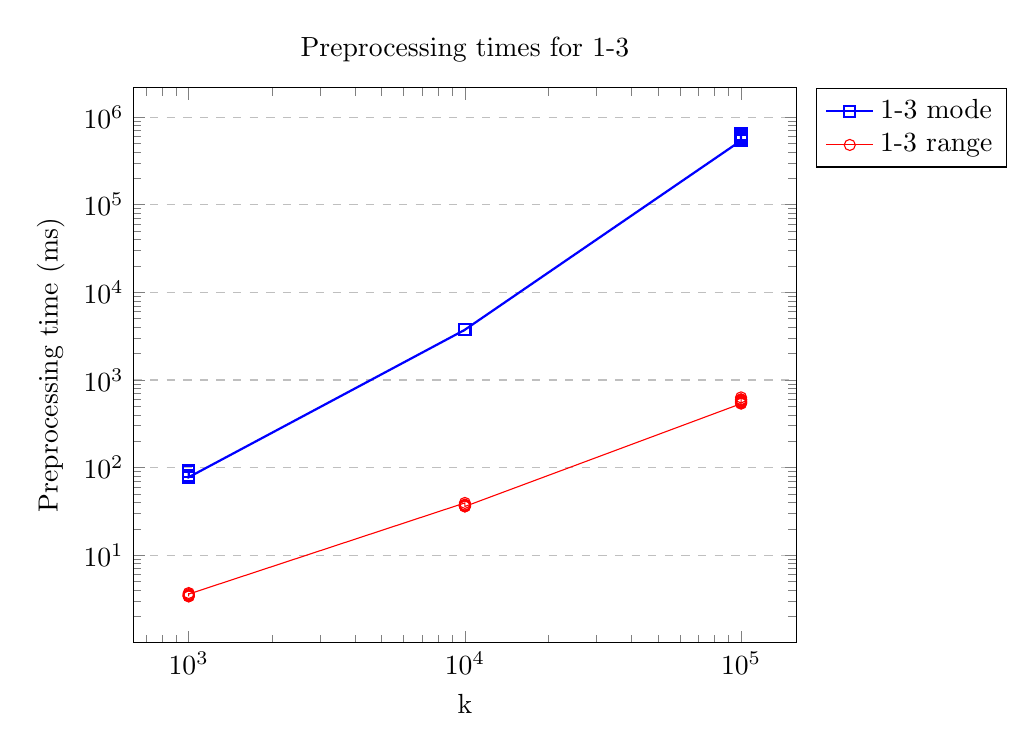
\begin{tikzpicture}
    \begin{axis}[
        title={Preprocessing times for 1-3},
        xmode=log,
        ymode=log,
        xlabel={k},
        ylabel={Preprocessing time (ms)},
        legend pos=outer north east,
        ymajorgrids=true,
        grid style=dashed,
    ]
    \addplot[
        color=blue,
        mark=square,
        thick,
        ]
        coordinates {
            (1000, 91.1)
            (1000, 78.1)
            (1000, 77.5)
            (1000, 76.5)
            (1000, 77.6)
            (1000, 80.6)
            (1000, 77.6)
            (10000, 3736.0)
            (10000, 3741.7)
            (10000, 3785.6)
            (10000, 3754.0)
            (10000, 3741.7)
            (10000, 3771.5)
            (10000, 3758.7)
            (10000, 3763.0)
            (10000, 3765.7)
            (10000, 3743.3)
            (100000, 539244.2)
            (100000, 579237.2)
            (100000, 599206.1)
            (100000, 589570.8)
            (100000, 559064.6)
            (100000, 569399.2)
            (100000, 609658.8)
            (100000, 639604.8)
            (100000, 549253.4)
            (100000, 559349.6)
        };
    \addlegendentry{1-3 mode}
    \addplot[
        color=red,
        mark=o,
        ]
        coordinates {
            (1000, 3.7)
            (1000, 3.4)
            (1000, 3.4)
            (1000, 3.5)
            (1000, 3.5)
            (1000, 3.4)
            (1000, 3.6)
            (10000, 39.5)
            (10000, 37.8)
            (10000, 36.9)
            (10000, 37.5)
            (10000, 37.2)
            (10000, 36.8)
            (10000, 36.2)
            (10000, 36.9)
            (10000, 36.2)
            (10000, 36.0)
            (100000, 536.5)
            (100000, 576.9)
            (100000, 595.2)
            (100000, 589.8)
            (100000, 559.8)
            (100000, 564.7)
            (100000, 601.9)
            (100000, 632.5)
            (100000, 544.9)
            (100000, 552.2)
        };
    \addlegendentry{1-3 range}
    \end{axis}
    \end{tikzpicture}
}
\resizebox{8cm}{!}{
    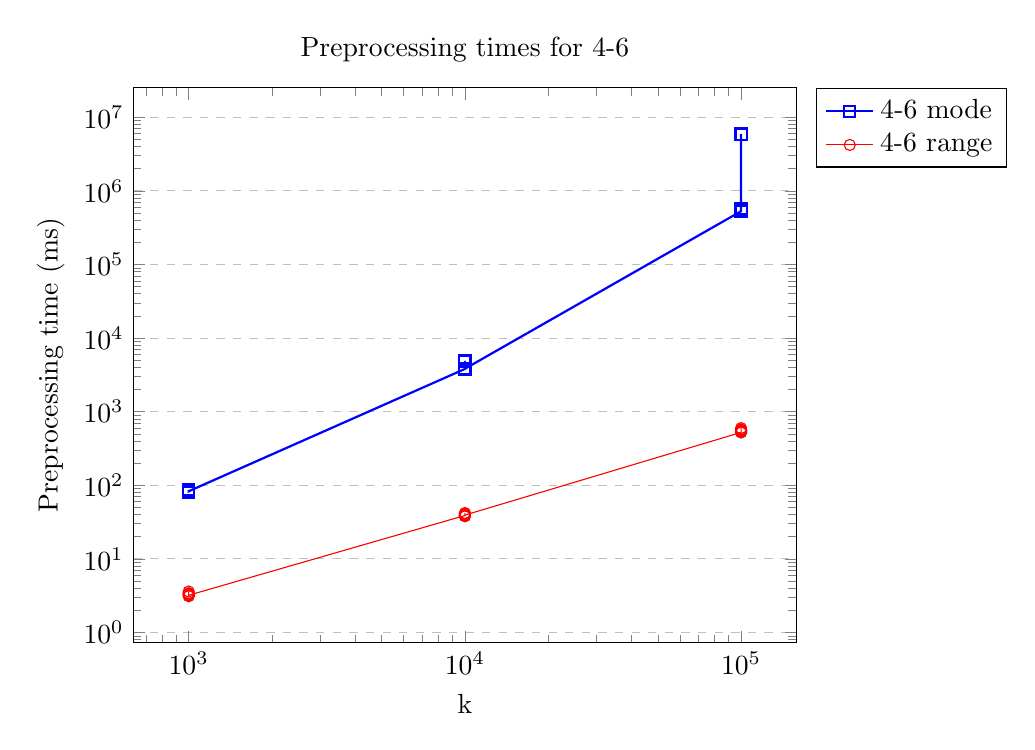
\begin{tikzpicture}
    \begin{axis}[
        title={Preprocessing times for 4-6},
        xmode=log,
        ymode=log,
        xlabel={k},
        ylabel={Preprocessing time (ms)},
        legend pos=outer north east,
        ymajorgrids=true,
        grid style=dashed,
    ]
    \addplot[
        color=blue,
        mark=square,
        thick,
        ]
        coordinates {
            (1000, 83.6)
(1000, 80.0)
(1000, 82.7)
(1000, 85.7)
(1000, 86.8)
(1000, 84.9)
(1000, 82.9)
(10000, 3802.2)
(10000, 3807.4)
(10000, 3790.2)
(10000, 3803.0)
(10000, 4857.3)
(10000, 3833.5)
(10000, 3895.0)
(10000, 4906.2)
(10000, 4892.9)
(10000, 3823.1)
(100000, 529303.1)
(100000, 538676.7)
(100000, 549054.4)
(100000, 559787.3)
(100000, 528902.3)
(100000, 539196.0)
(100000, 529283.1)
(100000, 5910225.5)
(100000, 569630.1)
(100000, 579868.2)
        };
    \addlegendentry{4-6 mode}
    \addplot[
        color=red,
        mark=o,
        ]
        coordinates {
            (1000, 3.4)
(1000, 3.2)
(1000, 3.3)
(1000, 3.4)
(1000, 3.6)
(1000, 3.1)
(1000, 3.2)
(10000, 38.8)
(10000, 37.8)
(10000, 38.4)
(10000, 38.3)
(10000, 40.8)
(10000, 38.6)
(10000, 39.0)
(10000, 41.2)
(10000, 41.9)
(10000, 39.3)
(100000, 522.6)
(100000, 535.1)
(100000, 547.6)
(100000, 552.5)
(100000, 527.2)
(100000, 533.6)
(100000, 525.2)
(100000, 598.5)
(100000, 569.6)
(100000, 573.8)
        };
    \addlegendentry{4-6 range}
    \end{axis}
    \end{tikzpicture}
}

\hskip-2cm
\resizebox{8cm}{!}{
    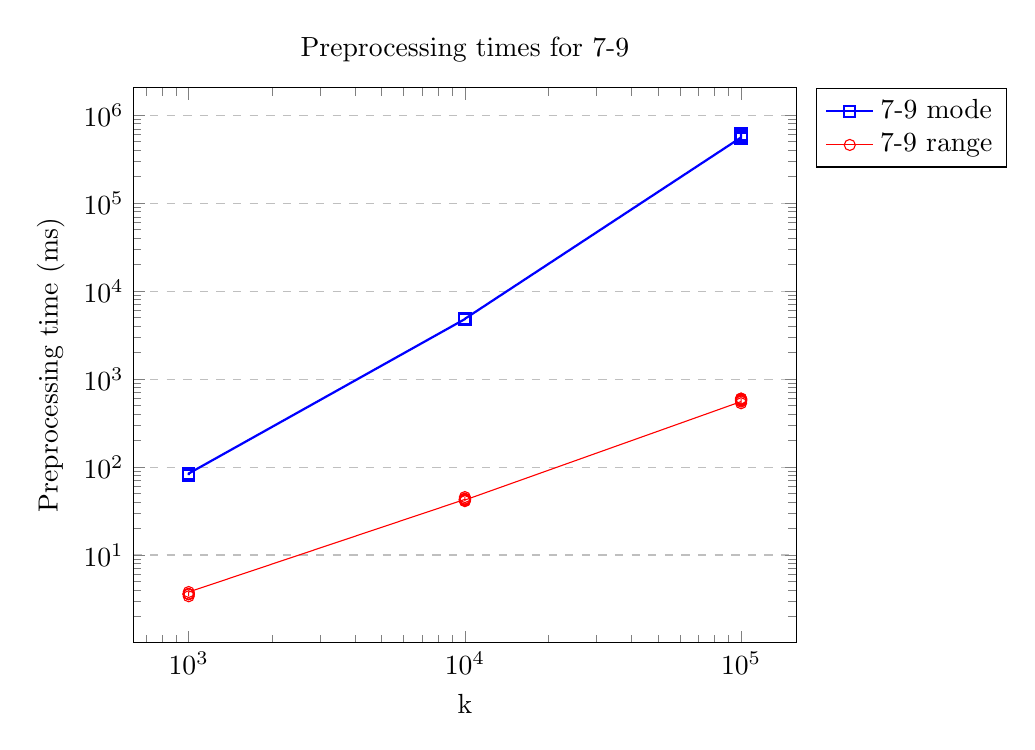
\begin{tikzpicture}
    \begin{axis}[
        title={Preprocessing times for 7-9},
        xmode=log,
        ymode=log,
        xlabel={k},
        ylabel={Preprocessing time (ms)},
        legend pos=outer north east,
        ymajorgrids=true,
        grid style=dashed,
    ]
    \addplot[
        color=blue,
        mark=square,
        thick,
        ]
        coordinates {
            (1000, 81.7)
(1000, 81.4)
(1000, 83.5)
(1000, 81.1)
(1000, 81.5)
(1000, 82.0)
(1000, 84.5)
(10000, 4811.7)
(10000, 4842.6)
(10000, 4844.6)
(10000, 4858.3)
(10000, 4859.4)
(10000, 4847.1)
(10000, 4879.8)
(10000, 4899.5)
(10000, 4848.3)
(10000, 4846.4)
(100000, 559095.2)
(100000, 599537.5)
(100000, 569218.3)
(100000, 599563.2)
(100000, 589237.1)
(100000, 579233.4)
(100000, 609799.3)
(100000, 589289.6)
(100000, 579136.4)
(100000, 538750.4)
        };
    \addlegendentry{7-9 mode}
    \addplot[
        color=red,
        mark=o,
        ]
        coordinates {
            (1000, 3.6)
(1000, 3.6)
(1000, 3.6)
(1000, 3.6)
(1000, 3.4)
(1000, 3.6)
(1000, 3.8)
(10000, 42.9)
(10000, 42.5)
(10000, 41.0)
(10000, 42.5)
(10000, 43.1)
(10000, 41.7)
(10000, 42.5)
(10000, 45.6)
(10000, 43.9)
(10000, 42.2)
(100000, 555.2)
(100000, 595.4)
(100000, 569.1)
(100000, 596.3)
(100000, 585.3)
(100000, 574.4)
(100000, 601.7)
(100000, 588.3)
(100000, 578.7)
(100000, 531.8)
        };
    \addlegendentry{7-9 range}
    \end{axis}
    \end{tikzpicture}
}
\resizebox{8cm}{!}{
    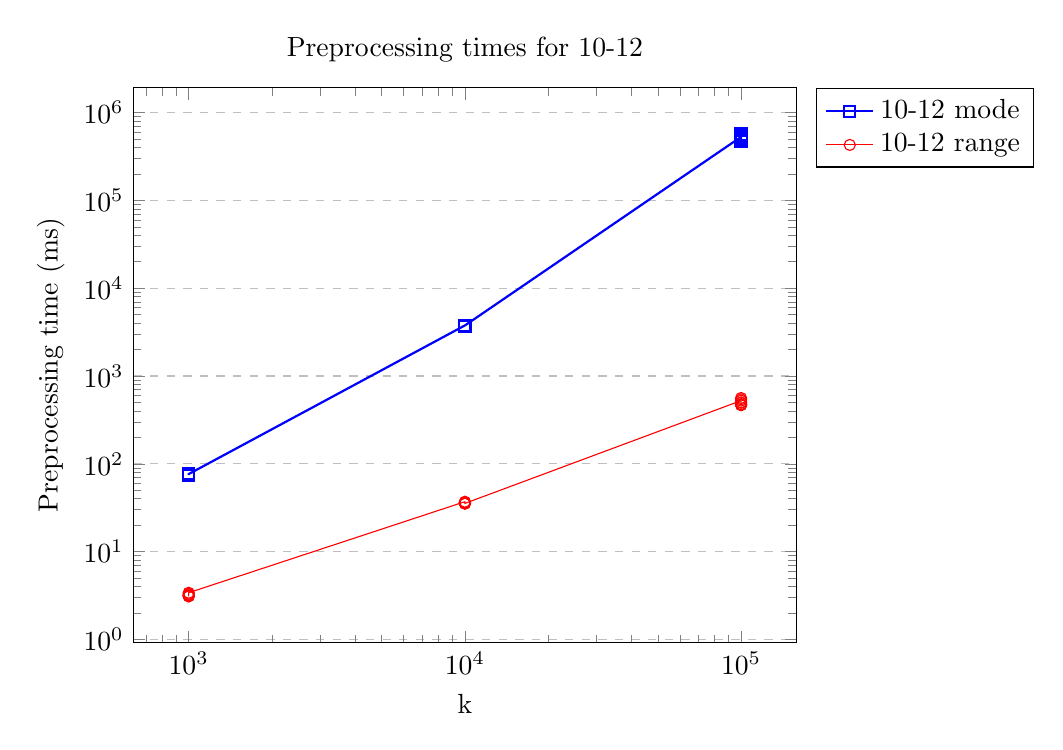
\begin{tikzpicture}
    \begin{axis}[
        title={Preprocessing times for 10-12},
        xmode=log,
        ymode=log,
        xlabel={k},
        ylabel={Preprocessing time (ms)},
        legend pos=outer north east,
        ymajorgrids=true,
        grid style=dashed,
    ]
    \addplot[
        color=blue,
        mark=square,
        thick,
        ]
        coordinates {
            (1000, 75.1)
(1000, 75.7)
(1000, 75.3)
(1000, 76.1)
(1000, 74.3)
(1000, 75.3)
(1000, 76.4)
(10000, 3767.2)
(10000, 3760.0)
(10000, 3763.3)
(10000, 3726.9)
(10000, 3712.3)
(10000, 3753.3)
(10000, 3750.5)
(10000, 3732.3)
(10000, 3754.3)
(10000, 3758.7)
(100000, 529238.8)
(100000, 498478.3)
(100000, 508609.6)
(100000, 569034.1)
(100000, 548548.0)
(100000, 478271.6)
(100000, 468515.4)
(100000, 478484.8)
(100000, 478319.6)
(100000, 468257.8)
        };
    \addlegendentry{10-12 mode}
    \addplot[
        color=red,
        mark=o,
        ]
        coordinates {
            (1000, 3.3)
(1000, 3.2)
(1000, 3.1)
(1000, 3.1)
(1000, 3.1)
(1000, 3.2)
(1000, 3.4)
(10000, 37.0)
(10000, 35.6)
(10000, 36.0)
(10000, 36.2)
(10000, 36.0)
(10000, 35.1)
(10000, 35.5)
(10000, 35.8)
(10000, 36.0)
(10000, 35.4)
(100000, 524.1)
(100000, 495.4)
(100000, 500.4)
(100000, 561.6)
(100000, 542.4)
(100000, 474.8)
(100000, 468.9)
(100000, 472.0)
(100000, 471.1)
(100000, 464.8)
        };
    \addlegendentry{10-12 range}
    \end{axis}
    \end{tikzpicture}
}

\subsubsection*{Discussion}
\fb{The range query results only somewhat match our expectations. When only looking at Figure \ref{fig:2dresrangeartificial}, the naive implementation seems to only be dependent on $n$, which could match the theoretical $O(n \log n)$ query time. Looking at Figure \ref{fig:2dresrangerl}a, we see a near linear relationship, which all but confirms the theoritical result. Of note is that for $n=1000$ in Figure \ref{fig:2dresrangeartificial}, the naive approach actually outperforms the fast implementation; we can therefore conclude that the hidden constant for our fast $O(\log n)$ approach must be rather large. \\\
The fast implementation does seem to have a slightly increased query time for larger $k$; this is best visible in Figure \ref{fig:2dresrangeartificial}b and is also the cause of the vertical spread in Figure \ref{fig:2dresrangerl}a. This anomaly was however explained when directly looking at the performance metrics in Visual Studio. We found here that for larger $k$, more time is spent querying large windows in our range tree. This in turn resulted in longer path traversals within the range tree, causing an increased runtime. As this seems to be the only source of computation time increase between small and large $k$ tests, we can therefore still conclude that our worst case is bounded by $O(\log^2 n)$. \\\\
When looking at mode queries, the results directly seem to match our expectations. In Figure \ref{fig:2dresmodeartificial}, we see that the naive implementation shows a linear relation with $k$ with different starting points for our smallest $k$, matching our $O(\log n + k)$ described algorithm. The query times of the fast implementation seem to be completely independent of $k$, thereby possibly matching our $O((n/r) \polylog n)$ query time. Looking at Figure \ref{fig:2dresmodeartificial}a we clearly see some dependency on $n$, and \ref{fig:2dresmodeartificial}b shows the inverse relationship with $r$. Due to the high dependence on $n$ it is hard to pinpoint an exact $k$ value at wich query times are lower than the naive approach, however it seems to be in the neighbourhood of $0.01n$ to $0.1n$.\\\\
Looking at only Figure \ref{fig:2drespreartificial}, preprocessing times for both the range and mode datastructures seem to follow a roughly linear relation with $n$. For the range datastructure this is no surprise, as the small number of sampled $n$ and scale of the graph would make it hard to see the $\log n$ factor that is included in the theoretical runtime. Additionally, as the default sorting method in C++ was used this might internally run faster than $O(n \log n)$ time by using something like a bucket sort approach depending on the input sequence. \\
As for the mode, this following a roughly linear relation is also expected. As $r$ was fixed for all these test cases currently considered, the linear relation matches the expected \fb{$O(nr^2)$} time. Only when we look at Figure \ref{fig:2dresprerl}b do we see the additional dependence on $r$. We once again note that this preprocessing time can most likely be reduced with a better implementation; as it stands, preprocessing for large $r$ is often not worth it due to the amount of queries that would be required to offset the initial workload.}
\section{Conclusion}
\fb{
    In this paper, we have succesfully implemented a selection of algorithms from van der Horst et al. \cite{vanderhorst_et_al:LIPIcs.ESA.2022.67}. In doing this, we showed that Chromatic $k$-Nearest Neighbours can be answered in a computationally efficient manner with no other dependence than the number of input points $n$, and have provided a base implementation that may be generalized to higher dimensions and other distance metrics. \\\\
    In our computational analysis, we see clear benefits from the approach proposed by van der Horst et al. In 1D, we see clear improvements in range query times when $k \gtrapprox 100$. For mode queries, we see similar behavior from $k \gtrapprox 300$, thereby allowing us to conclude that the methods implemented might greatly increase performance when compared to naive approaches when $k$ is large. \\
    For 2D we achieve similar results, with a breakeven point for range queries at around $n=2000$ (regardless of $k$). For mode queries, we implemented a modified version of the algorithm which returns halfplane queries instead; this also outperforms the naive approach when $k$ is around $0.01n$ to $0.1n$, once again making it useful when $k$ is large. \\\\
    Some things of note can still be directly improved in our implementation. For 2D mode finding specifically, we deviated both from the theoretically optimal running time as well as space usage by using a naive approach for handling conflict lists. Implementing the improvements described in the original paper here could drastically decrease the preprocessing time of the algorithm, thereby allowing larger $r$ values to be used for even lower query times. If feasible, this would also allow for the theoretical $r=\sqrt{n}$ to be used. Secondly, the implementation as a whole can probably still be improved. More agressive compiler optimizations can still be used given some more testing, and due to a lack of experience with C++11 and CGAL some additional possibilities for speedup were likely overlooked. \\\\
    Due to time constraints, something that was left out of testing was handling of all edge cases within the implementation. Especially for the 2D implementation, testing should still be done using duplicate data points, overlapping query and data points and grid-like datasets in which x and y coordinates are strictly not unique to validate that the correct result is still returned. In addition to this, experiments may be run with different numerical data types in CGAL in order to quantify the performance decrease associated with higher precision point locations and line intersections. \\\\
    Finally, once 3D arrangements are available further experimentation should also be done in order to fully implement 2D mode finding. This can then be used in order to generalize to higher dimensions, as well as solving inherent limitations present in the halfspace queries such as a small central clusters of points never being a mode candidate. \\\\
}
    
\printbibliography
\end{document}
